\documentclass{article}
\usepackage{beamerarticle}

\usepackage{tcolorbox}
\tcbuselibrary{breakable}

\renewtcolorbox{block}[1]{
    /utils/exec={\if\relax\detokenize{#1}\relax\else\pgfkeysalso{title={#1}}\fi},
    breakable,
    colback=white,
    colframe=black!30,
    colbacktitle=black!10,
    coltitle=black,
    fonttitle=\bfseries,
    boxrule=0.5pt,
    arc=2pt
}

% Theme choice (you can change to Madrid, CambridgeUS, etc.)
\usetheme{Madrid}

% Optional packages
\usepackage[utf8]{inputenc}
\usepackage{graphicx} % for including images
\usepackage{amsmath, amssymb, mathtools} % for math symbols
\usepackage{hyperref} % for clickable links
\usepackage{xurl}
\usepackage{tikz}
\usepackage{listings}
\usepackage{xstring}

\usetikzlibrary{positioning}

% Title info
\title{Latency}
\author{Oden Petersen}
\date{2026-09-23}


% Section headers
\newif\ifhasdiagram
\hasdiagramfalse

\newcommand{\sectiondiagram}[1]{%
    \def\insertsdiagram{#1}%
    \hasdiagramtrue
}

\newcommand{\sectionquote}[1]{%
    \def\insertsquote{\small #1}%
}

\newcommand{\insertsdiagram}{}
\newcommand{\insertsquote}{}

\let\oldsection\section
\RenewDocumentCommand{\section}{s o m}{%
    \IfBooleanTF{#1}{\oldsection*{#3}}{\IfValueTF{#2}{\oldsection[#2]{#3}}{\oldsection{#3}}}%
    {\centering\insertsquote\par}%
    \renewcommand{\insertsquote}{}%
}

% Diagram
\newcommand{\diagram}[1]{%
    \begin{center}
    \begin{tikzpicture}[
        >=stealth,
        box/.style={
            draw,
            minimum width=2.2cm,
            minimum height=.7cm
        },
        hi/.style={fill=gray!25, thick}
    ]

        \newcommand{\N}[3]{%
            \IfStrEq{#1}{##1}
                {\node[box,hi] (##1) at (##2) {##3};}
                {\node[box] (##1) at (##2) {##3};}%
        }

        % Main cycle
        \N{matching}{0,0}{Matching Engine}
        \N{execution}{-3,-1}{Execution}
        \N{market}{3,-1}{Market Data}
        \N{network}{0,-2}{Network Interface}

        % Hardware / software
        \N{hardware}{0,-3.5}{Hardware}
        \N{software}{0,-5}{Software}
        \N{program}{3,-5}{Program}

        % Main cycle
        \draw[->] (execution.east) -- (matching.south);
        \draw[->] (matching.south) -- (market.west);
        \draw[->] (market.west) -- (network.north);
        \draw[->] (network.north) -- (execution.east);

        % Network / hardware
        \draw[->] (network.south) to[bend left=15] (hardware.north);
        \draw[->] (hardware.north) to[bend left=15] (network.south);

        % Hardware / software
        \draw[->] (hardware.south) to[bend left=15] (software.north);
        \draw[->] (software.north) to[bend left=15] (hardware.south);

        % Program
        \draw[->] (program.west) -- (software.east);

    \end{tikzpicture}
    \end{center}%
}

\begin{document}

\maketitle

\begin{center}
	``I think you should know one level well, have a working knowledge of the level beneath you, and then \ldots be aware of the shape of the layer beneath that.'' Matt Godbolt
\end{center}

No AI writing has been used here, with the exception of some of the code, plots, and formatting. This is the result of reading and experience.

I originally presented this as a talk to around 25 students and alumni at UNSW.

Links: \textcolor{blue}{\href{https://github.com/odenpetersen/trading-presentation}{GitHub Repo, Other Talks}}, \textcolor{blue}{\href{https://www.youtube.com/watch?v=GHZncZyFnqo}{Talk Recording}} (2h11m), \textcolor{blue}{\href{http://linkedin.com/in/oden-petersen}{About me}}
\section*{Overview}
This work will give an overview of electronic trading and the various networking and processing devices involved. The emphasis is on where latency comes from and how to design fast systems. I will also cover some more general computer science topics with trading as the motivation.

There will be a lot of general principles. In practice, specifics matter a great deal, and as a consequence are usually not widely shared.

The work is in three parts.

\textbf{Part I} will provide motivation and give an overview of some prerequisite concepts.

\textbf{Part II} analyses the networking components present in an exchange colocation.

\textbf{Part III} discusses the design of systems to quickly react to exchange data.

\subsection*{How To Use These Notes}
Both the talk and the notes cover a lot and are quite long. I would recommend checking the table of contents to see which parts might be most interesting to you.

The raw information is mostly all presented here. In the talk I give various demos, code examples, etc., particularly for the hardware and software design components. The slides are labeled very similarly to the table of contents so hopefully you can quickly find the relevant part of the recording.

\newpage

\setcounter{tocdepth}{3}
\tableofcontents

\part{Concepts}
\sectionquote{``All economic activity is carried out through time. Every individual economic process occupies a certain time, and all linkages between economic processes necessarily involve longer or shorter periods of time.'' Friedrich Hayek}
\section{Trading}

\subsection{Electronic Trading}
Electronic trading involves interacting with a \textbf{matching engine}.
\begin{block}{Limit Order Book}
	A \textbf{limit order} represents an intention to trade some \textbf{quantity} in some \textbf{direction} at some \textbf{limit price} or better.


	\begin{itemize}
	\item We can send three kinds of messages to the matching engine:
	\begin{itemize}
	\item \textbf{Insert} an order with some \textbf{lifetime} (e.g. GTC, GFD, FAK, FOK)
	\item \textbf{Cancel} or \textbf{modify} existing order(s)
	\end{itemize}
	\end{itemize}

	The matching engine maintains an \href{https://www.binance.com/en-AU/trade/BTC_USDT}{\textbf{order book}} and produces \textbf{matches} when two orders are willing to trade with each other.
\end{block}

A market is a distributed computer for producing trades at mutually agreeable prices.

\subsection{Trading Strategies}
\begin{block}{Arbitrage}
	\textbf{Arbitrage} refers to making offsetting trades in different order books, like buying a stock on one exchange and selling it on another. For instance, we might buy an ETF at some price and sell an equivalent future at a higher price. In principle the risks of these two assets should offset perfectly.

	This often involves a \textbf{race condition}, with the risk of getting `\textbf{legged}' (e.g. buying the ETF but failing to sell the future).
\end{block}

\begin{block}{Risk}
	The other way to make money involves taking on risk.

	\textbf{Statistical Arbitrage} involves positions that might not offset perfectly, such as futures on different indices.

	\textbf{Speculation} involves making a trade with the expectation of offsetting it at some later time.

	Traders have varying \textbf{risk profiles}, which causes disagreement about which trades are favourable.

	The more favourable trades we have access to, the more we can make, and the faster we can trade out of a risky position. This has a similar effect to that of liquidity on the riskiness of a position.
\end{block}

\subsection{Toy model}
Expected quadratic utility of trading $q$ units with a forecast horizon $h$, forecast $\mu$, volatility $\sigma$, and risk aversion $\lambda$ is roughly given by
$$q \mu-\lambda q^2 \sigma^2(h+t),$$
where $t$ is the time taken to get out of the position at a fair price.

\subsection{Low-Latency Trading}
Access to a bigger set of trades, and understanding of how to make use of this access, represents a concrete, measurable edge. Almost any profitable trading strategy can be improved by being faster.

Latency helps the most with the most competitive opportunities.

Very large trading businesses may become less latency-focused as risk budgets expand due to capacity constraints. However, market structure understanding remains relevant for understanding and classifying order flow.

\subsection{Empirical Analysis: SPY on NYSE}
This will serve to illustrate some basic concepts.

I took market data PCAPs from NYSE and parsed them to evaluate two different trading strategies on the SPY ETF (before fees):
\begin{enumerate}
	\item Whenever we see a trade, insert a one-lot FAK in the same direction at the same level
	\item Whenever we see a trade, insert a one-lot FAK in the same direction one tick behind the traded level
\end{enumerate}
If the triggering trade has already taken all the liquidity, we don't send an order.

Both of these are pretty dumb and won't make money.

Among the pool of opportunities, here's the CDF of how long it takes for the liquidity we are trying to trade against to disappear.
\begin{center}
	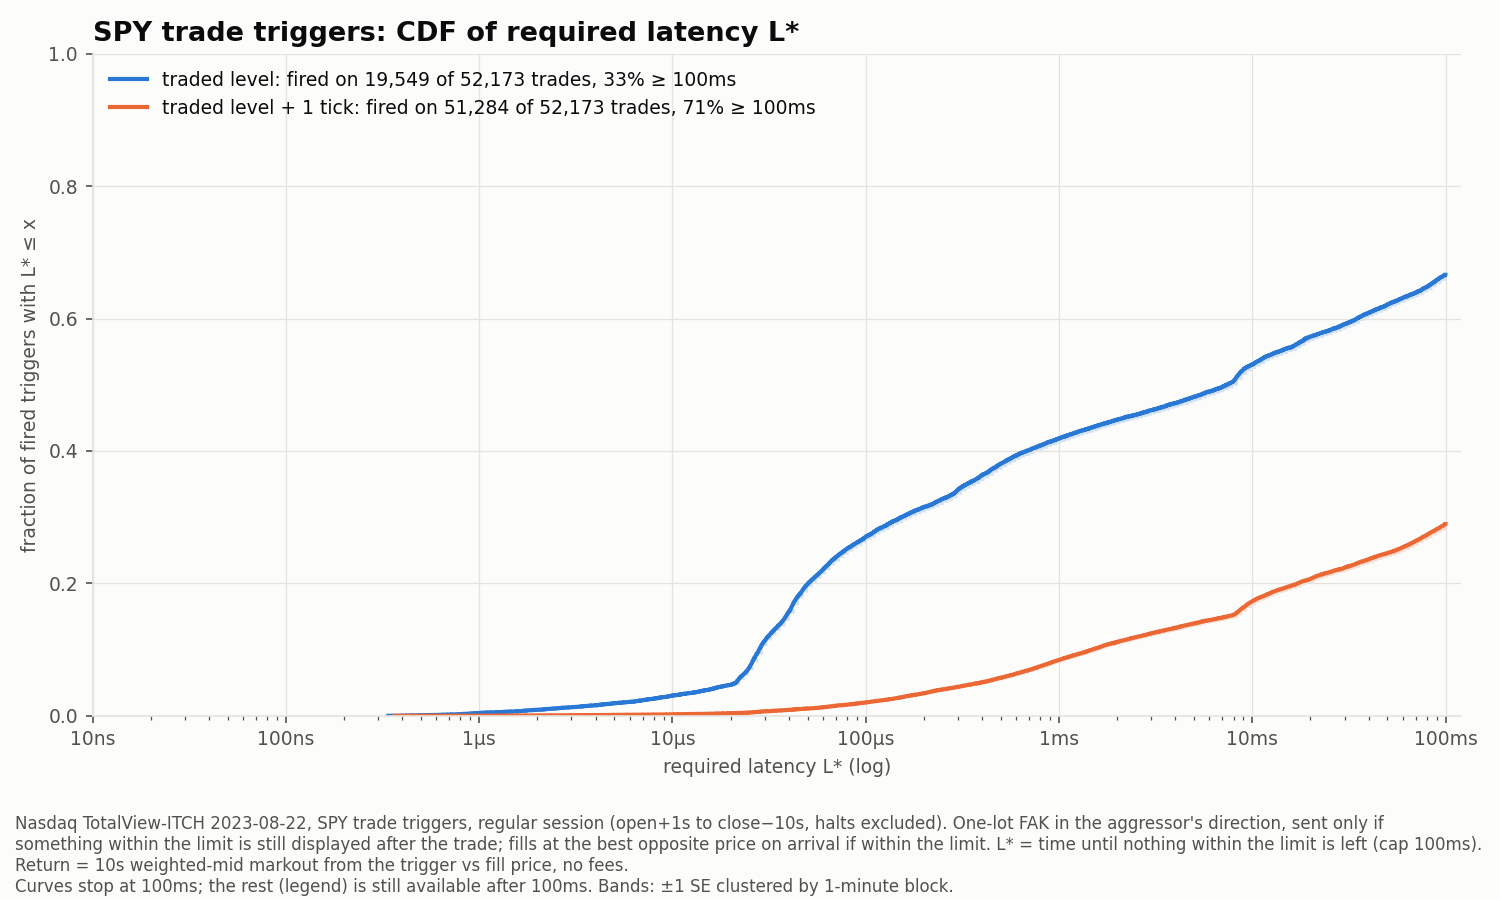
\includegraphics[scale=0.45]{assets/latency_cdf.png}
\end{center}
We can be slower if we are more aggressive with our prices.

Similarly, we can look at fill rate. This is not exactly equivalent, because there is an edge case where the liquidity refills before our order arrives.

I use four different of latency models parameterised by the mean: constant latency, and then three families of normally distributed latency models with different standard deviation.
\begin{center}
	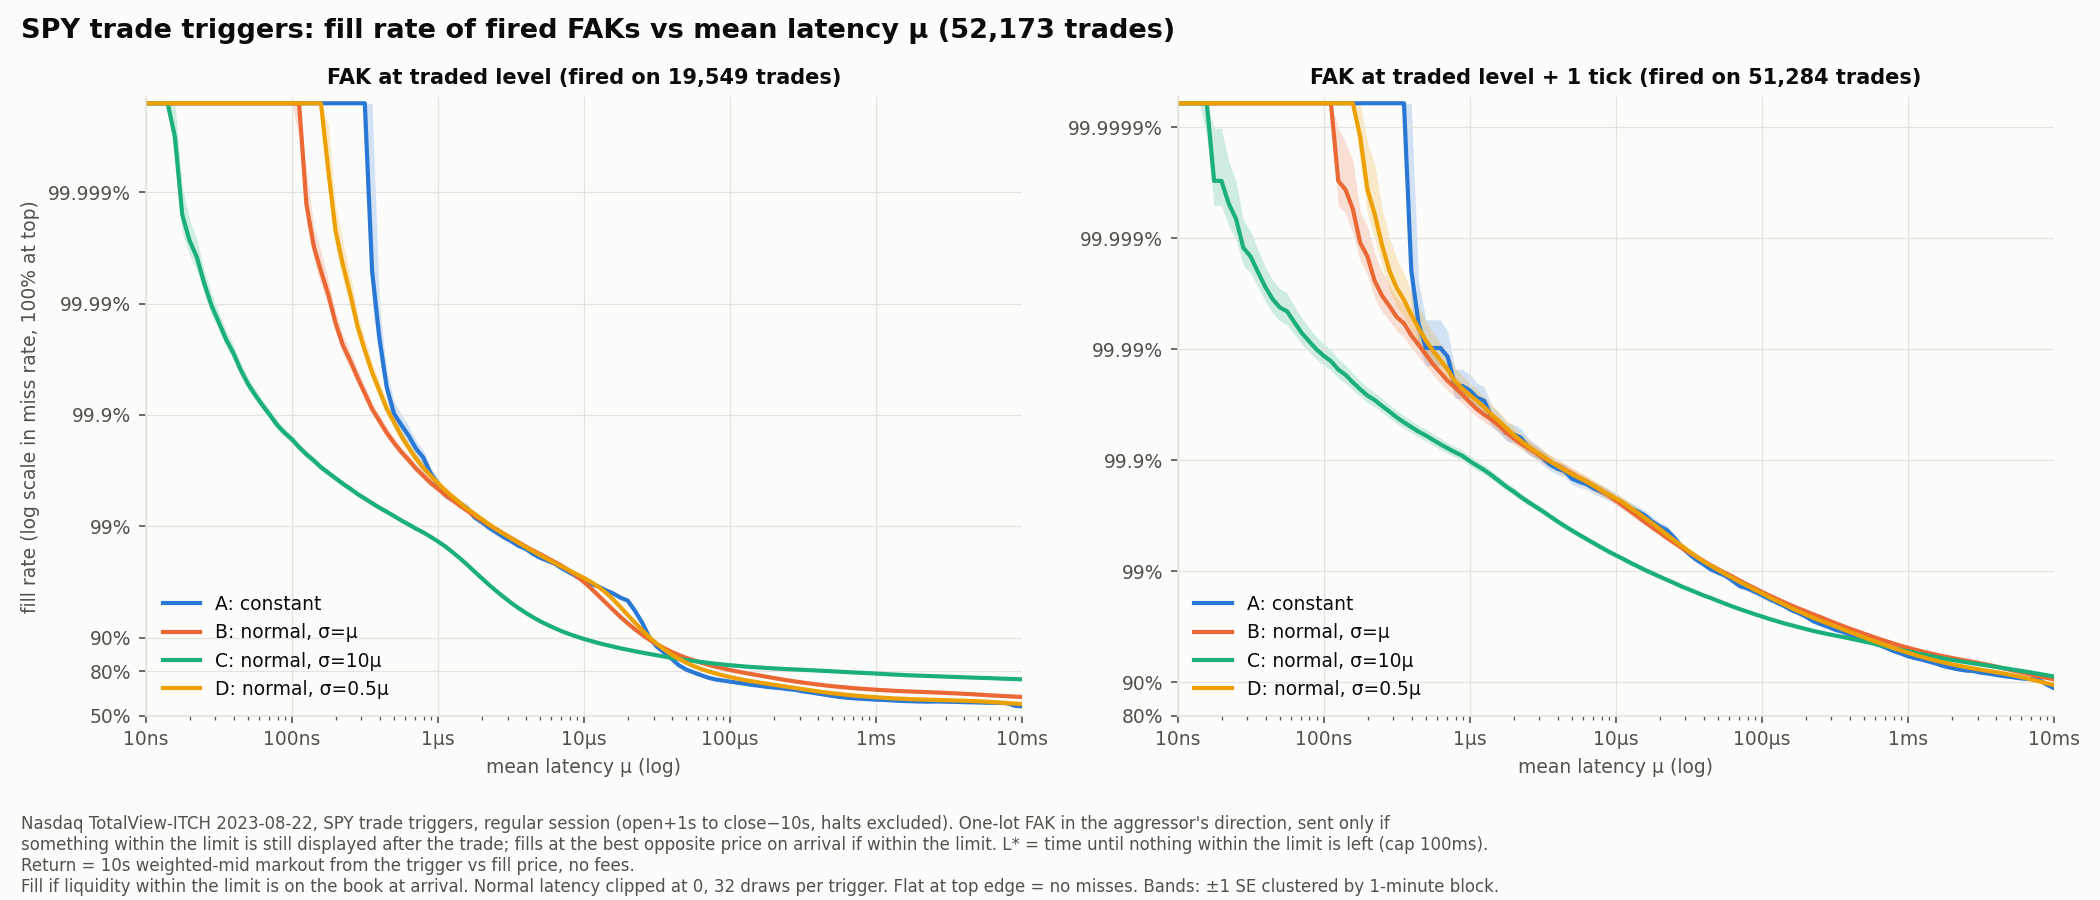
\includegraphics[scale=0.35]{assets/fill_rate.png}
\end{center}
Fill rate should generally go down as we get slower.

Finally, we can look at mean returns (ignoring fees) on a 10-second horizon (marked to weighted midprice).
\begin{center}
	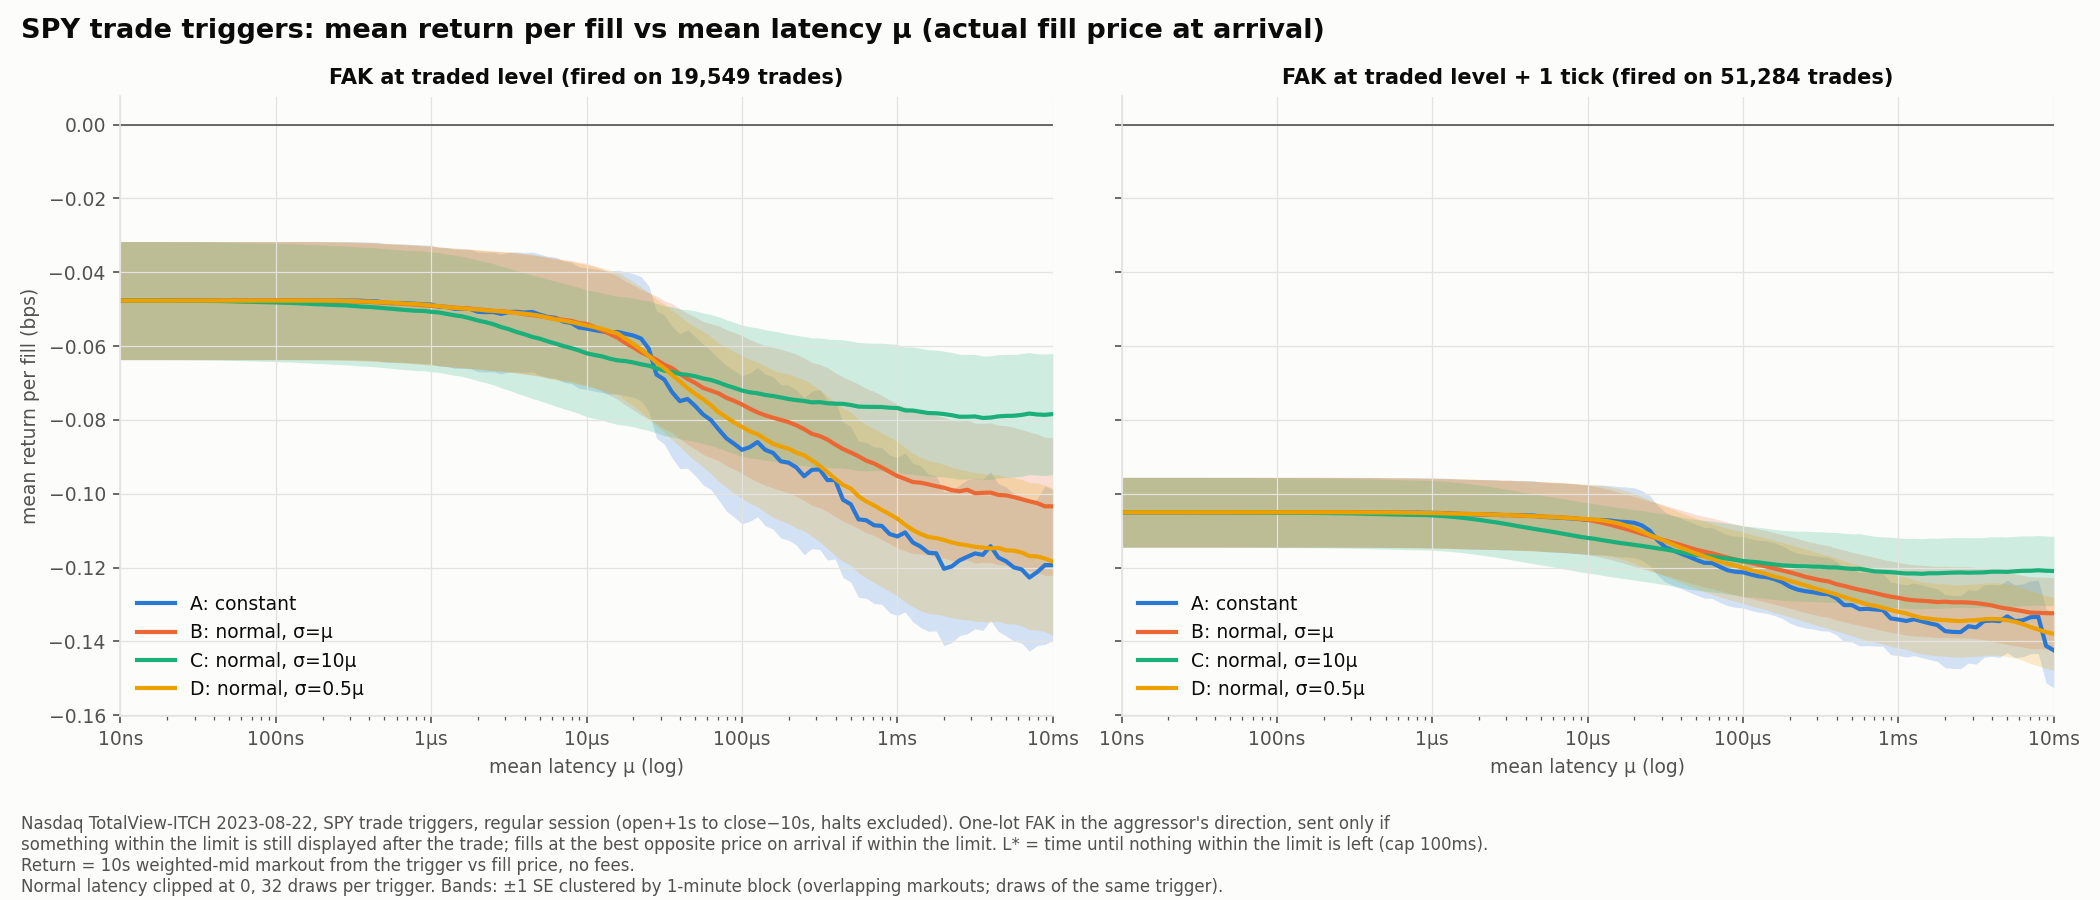
\includegraphics[scale=0.35]{assets/return_per_fill.png}
\end{center}
Standard error is computed from the population of trades we actually get filled on.

We can see that returns degrade as we get slower. This represents adverse selection.

We also see that jitter is helpful when the constant-latency curve is convex and harmful when it is concave (as a consequence of Jensen's inequality).

\subsection{Latency}
Latency is the delay between two events. For instance, we can look at the delay between sending a ping and receiving the response.

Here's on my home network:
\begin{lstlisting}[ basicstyle=\ttfamily\bfseries\scriptsize ]
> date +%s%N
1788413610858617734
\end{lstlisting}
Epoch timestamp:
\begin{math}
	\underbrace{1788413610}_{\text{epoch seconds}}\underbrace{858}_{\text{millis}} \underbrace{617}_{\mu\text{s}} \underbrace{734}_{\text{nanos}}
\end{math}
\begin{lstlisting}[ basicstyle=\ttfamily\bfseries\scriptsize ]
> ping -c 5 192.168.0.109
PING 192.168.0.109 (192.168.0.109): 56 data bytes
64 bytes from 192.168.0.109: icmp_seq=0 ttl=64 time=3.763 ms
64 bytes from 192.168.0.109: icmp_seq=1 ttl=64 time=5.376 ms
64 bytes from 192.168.0.109: icmp_seq=2 ttl=64 time=7.845 ms
64 bytes from 192.168.0.109: icmp_seq=3 ttl=64 time=43.958 ms
64 bytes from 192.168.0.109: icmp_seq=4 ttl=64 time=4.174 ms

--- 192.168.0.109 ping statistics ---
5 packets transmitted, 5 packets received, 0.0% packet loss
round-trip min/avg/max/stddev = 3.763/13.023/43.958/15.533 ms
\end{lstlisting}

Hopefully later sections will explain some of the sources of the variance here.

\sectionquote{``Time \ldots is what keeps everything from happening at once.'' Ray Cummings \\ 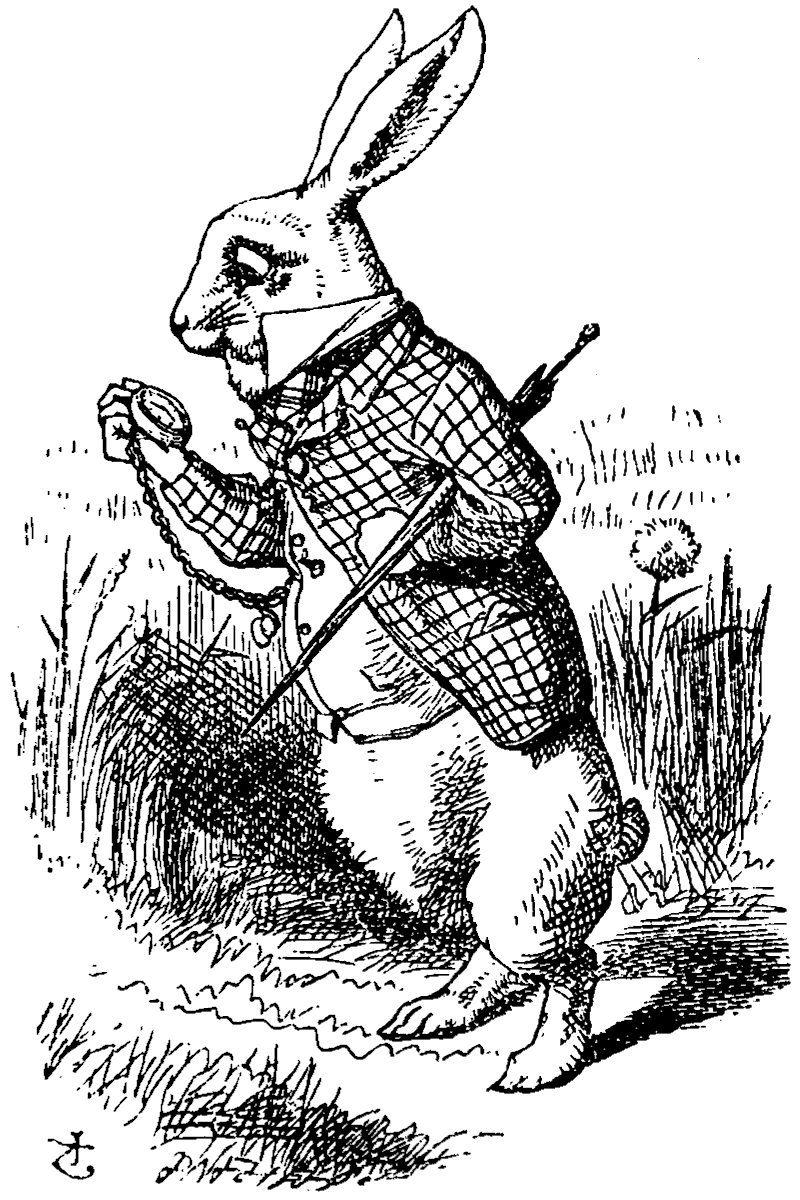
\includegraphics[scale=0.4]{assets/rabbit.png} \\ ``By a clock we understand anything characterized by a phenomenon passing periodically through identical phases so that \ldots all that happens in a given period is identical with all that happens in an arbitrary period.'' Albert Einstein}%16MHz
\section{Time}

\subsection{Clocks}
Quartz powered by a DC signal vibrates due to the piezoelectric effect at a reliable \textbf{reference frequency}.
	\begin{center} 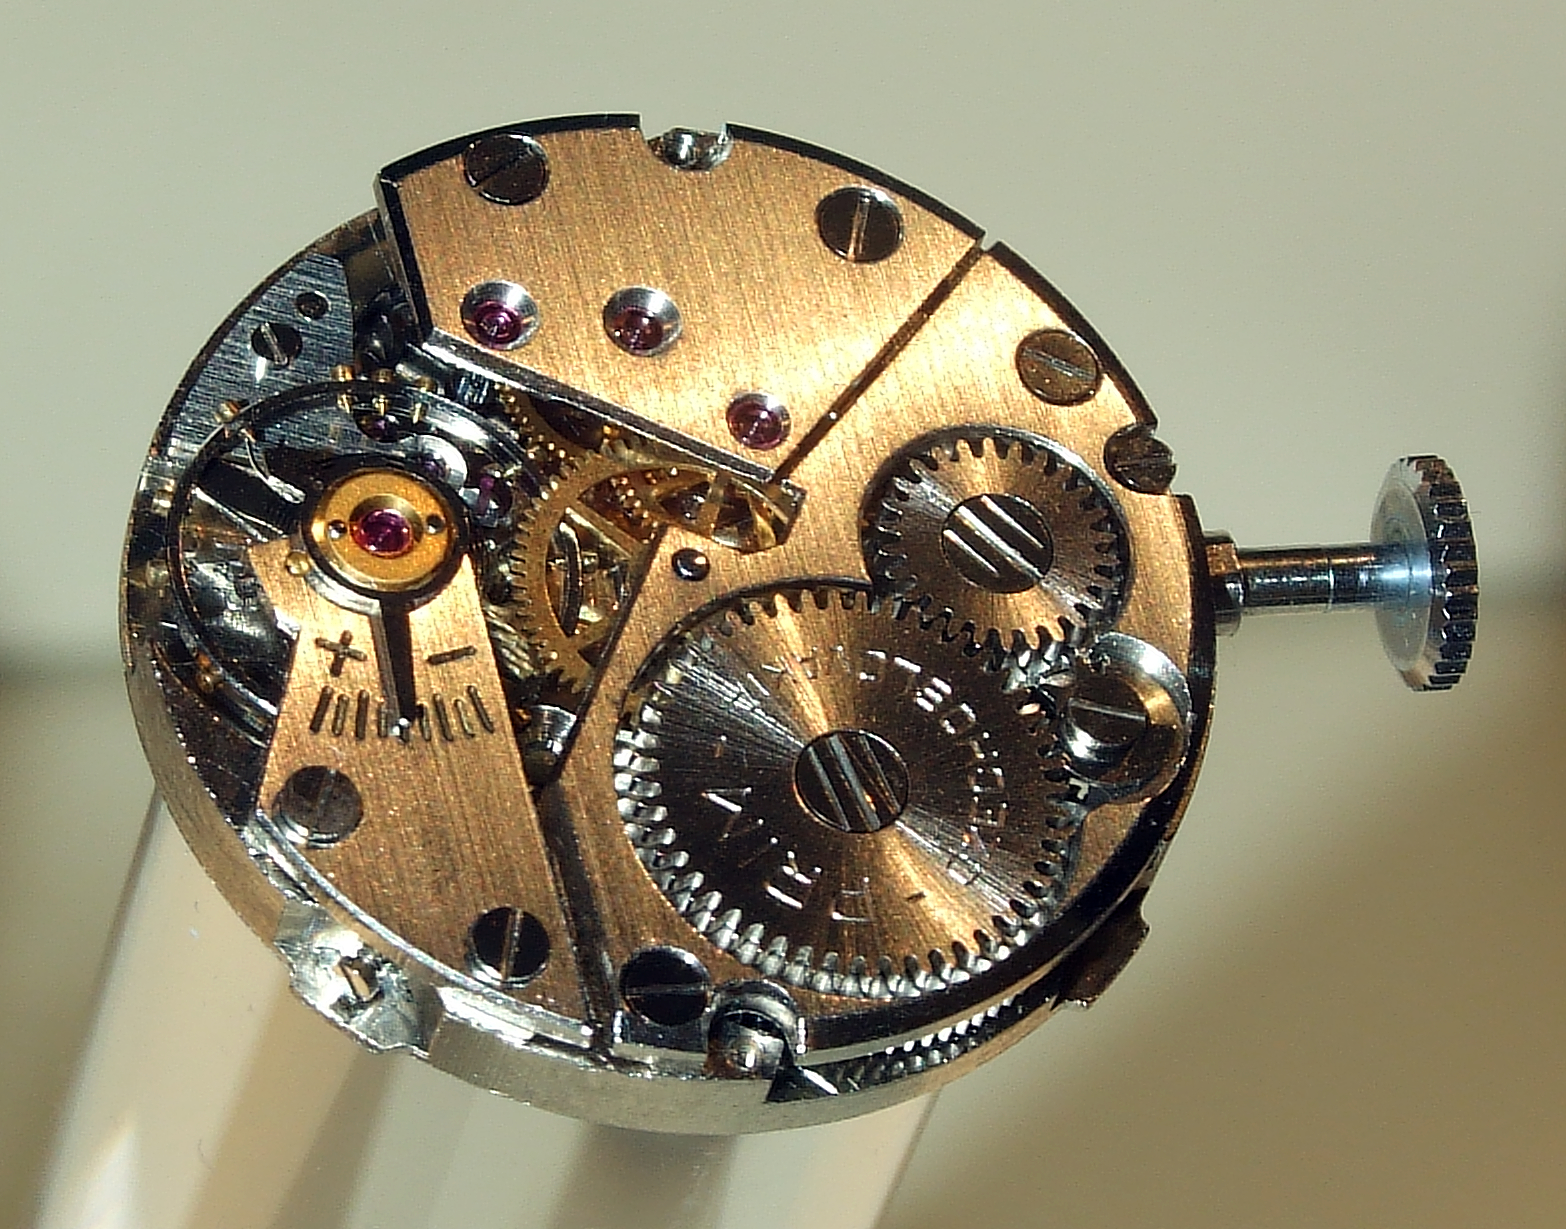
\includegraphics[scale=0.04]{assets/clockwork.jpg} 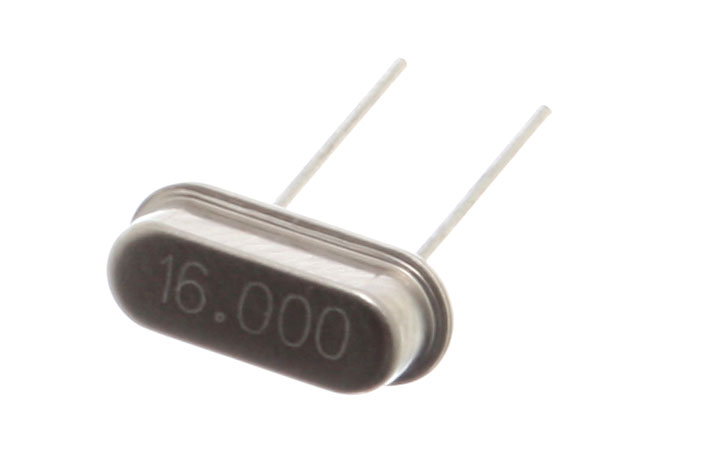
\includegraphics[scale=0.2]{assets/crystal.jpg} \end{center}
A \textbf{voltage-controlled oscillator} has a frequency dependent on the input voltage.

A \textbf{phase detector} can produce a signal whose strength depends on how fast or slow the VCO is running compared to the reference.

By keeping the VCO in a \textbf{phase-locked loop} with the reference, we can achieve oscillation at some multiple of the reference frequency. This can be chained a number of times.

\subsubsection{Clock Drift}
Heat, manufacturing differences, crystal aging, voltage fluctuations, etc., can cause two clocks $T_1(t)$ and $T_2(t)$ to experience \textbf{clock drift}, whereby $\theta_{1\to 2} = T_2(t)-T_1(t)$ changes over time.

Here's the lowest quartile of the difference between receipt timestamps and match timestamps for NYSE, in 30min buckets. I only consider packets with a single message pertaining to SPY (other symbols may be on a different clock).
\begin{center}
	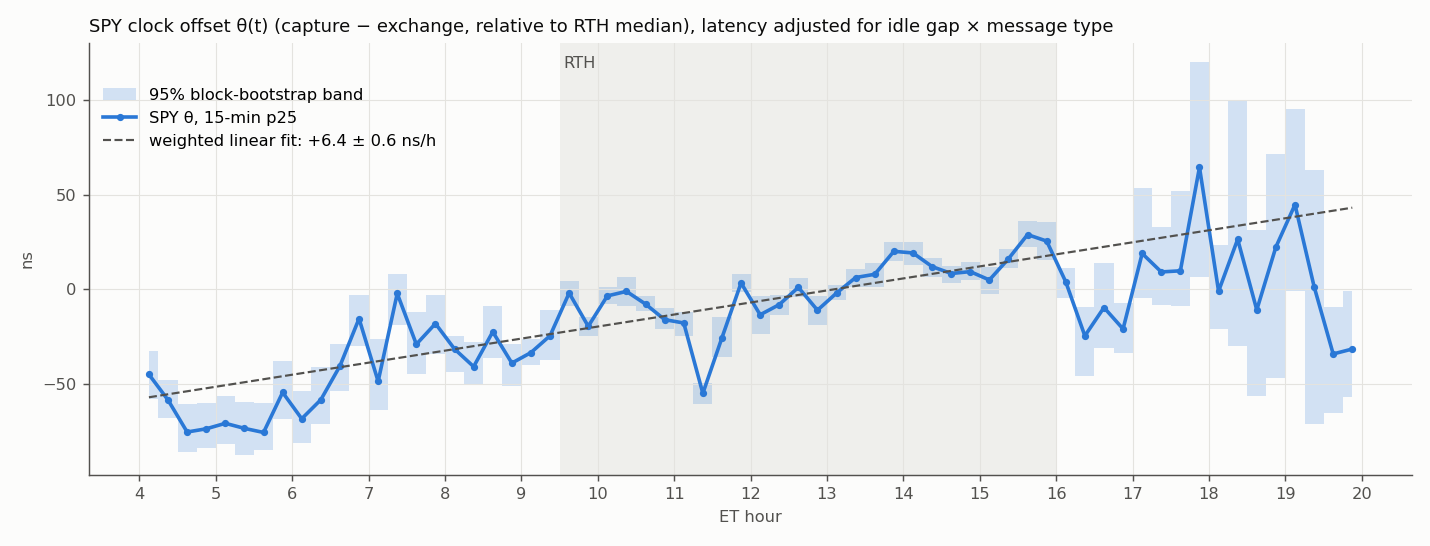
\includegraphics[scale=0.4]{assets/clock_drift.png}
\end{center}

It is possible to observe negative apparent latency when naively comparing timestamps from poorly synced clocks.

Note that in theory this could also be explained by gradual changes in service quality.

\subsection{Synchronisation}
For synchronisation within a network we will typically have a time server with a \textbf{master clock}. This could be set just once or synced with some external source like GPS.

\begin{center}
	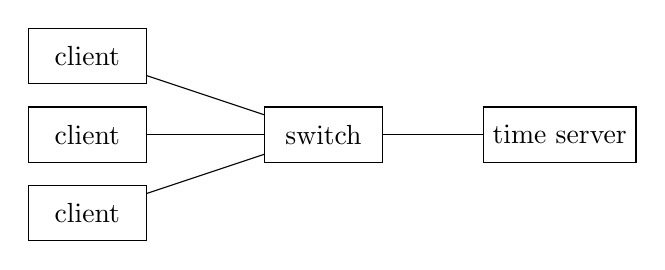
\begin{tikzpicture}[
	    node distance=2cm,
	    every node/.style={draw, rectangle, minimum width=1.5cm, minimum height=0.7cm}
	]
	    \node (switch) at (0,0) {switch};
	    \node (master) at (3,0) {time server};

	    \foreach \y in {1,0,-1} {
		\node (client\y) at (-3,\y) {client};
		\draw (client\y) -- (switch);
	    }

	    \draw (switch) -- (master);
	\end{tikzpicture}
\end{center}

\begin{block}{Clock Drift Estimation}
	Each piece of hardware can be equipped with its own clock $T_{*}(t)$.

	We can \textbf{send messages} over the network, \textbf{record timestamps} at each device clock, and \textbf{adjust for latency}.

	This allows us to adjust the client clock speed (\textbf{slewing}) such that $\theta_{c\to m}$ approaches zero.
\end{block}

\subsubsection{Network Time Protocol}
Using the \textbf{network time protocol} involves the client making requests to the time server that are labeled with four receive/transmit timestamps $T_c(t_1), T_m(t_2), T_m(t_3), T_c(t_4)$.

Suppose we have symmetric latency $T_m(t_2)-T_m(t_1) = T_m(t_4)-T_m(t_3)$.
It follows that $T_m(t_2)-(T_c(t_1)+\theta_{c\to m}) = (T_c(t_4)+\theta_{c\to m})-T_m(t_3)$. Then
\begin{align*}
	\theta_{c\to m} &= \frac{1}{2}\left(\underbrace{(T_m(t_2)-T_c(t_1))}_\text{Transmit} - \underbrace{(T_c(t_4)-T_m(t_3))}_\text{Receive}\right) \\
	&= \underbrace{\frac{1}{2}(T_m(t_3)+T_m(t_2))}_{\text{Midpoint for }m} - \underbrace{\frac{1}{2}(T_c(t_4)+T_c(t_1))}_{\text{Midpoint for }c} \\
\end{align*}

In the case where wire-to-wire latency is zero, this is also known as Einstein synchronisation.

\subsubsection{Precision Time Protocol}
Because the latency added by a switch is nondeterministic, we can achieve greater precision by controlling for its contribution.

Suppose we have $T_c(t_1), T_s(t_2), T_s(t_3), T_m(t_4), T_m(t_5), T_s(t_6), T_s(t_7), T_c(t_8)$.

Then we have
$$\theta_{c\to s} = \frac{1}{2}\left((T_s(t_2)-T_c(t_1)) - (T_c(t_8)-T_s(t_7))\right),$$
$$\theta_{s\to m} = \frac{1}{2}\left((T_m(t_4)-T_s(t_3)) - (T_s(t_6)-T_m(t_5))\right),$$
$$\theta_{c\to m} = \theta_{c\to s} + \theta_{s\to m}.$$

We can either record a cumulative adjustment in the timing packets (\textbf{transparent clock}), or sync the switch to the master clock and then the client to the switch (\textbf{boundary clock}).

\sectionquote{``Speed is the essence of war.'' Sun Tzu \\ ``Remote fountains are of little help to nearby fires.'' Han Fei}
\section{Distance}
A lot of sources of latency are ultimately reducible to distance.

\subsection{Wide Area Networking}
\subsubsection{Internetworking}
Things that are further away usually take longer to get a reply from.

This is on my home network:
\begin{lstlisting}[ basicstyle=\ttfamily\bfseries\scriptsize ]
> ping -c 3 192.168.0.109
PING 192.168.0.109 (192.168.0.109): 56 data bytes
64 bytes from 192.168.0.109: icmp_seq=0 ttl=64 time=2.593 ms
64 bytes from 192.168.0.109: icmp_seq=1 ttl=64 time=12.022 ms
64 bytes from 192.168.0.109: icmp_seq=2 ttl=64 time=53.092 ms

--- 192.168.0.109 ping statistics ---
3 packets transmitted, 3 packets received, 0.0% packet loss
round-trip min/avg/max/stddev = 2.593/22.569/53.092/21.924 ms
\end{lstlisting}

This is in London:
\begin{lstlisting}[ basicstyle=\ttfamily\bfseries\scriptsize ]
> ping -c 3 46.17.63.250
PING 46.17.63.250 (46.17.63.250): 56 data bytes
64 bytes from 46.17.63.250: icmp_seq=0 ttl=30 time=403.366 ms
64 bytes from 46.17.63.250: icmp_seq=1 ttl=30 time=338.468 ms
64 bytes from 46.17.63.250: icmp_seq=2 ttl=30 time=336.076 ms

--- 46.17.63.250 ping statistics ---
3 packets transmitted, 3 packets received, 0.0% packet loss
round-trip min/avg/max/stddev = 336.076/359.303/403.366/31.172 ms
\end{lstlisting}

Alternative data sources often need to travel over the public internet.

\subsubsection{Private Wide Area Network Links}
1850: Paul Reuter establishes a carrier pigeon service between financial hubs in Germany and Belgium

2010: Spread Networks lays a private (`dark') optic fiber network between Chicago and New Jersey

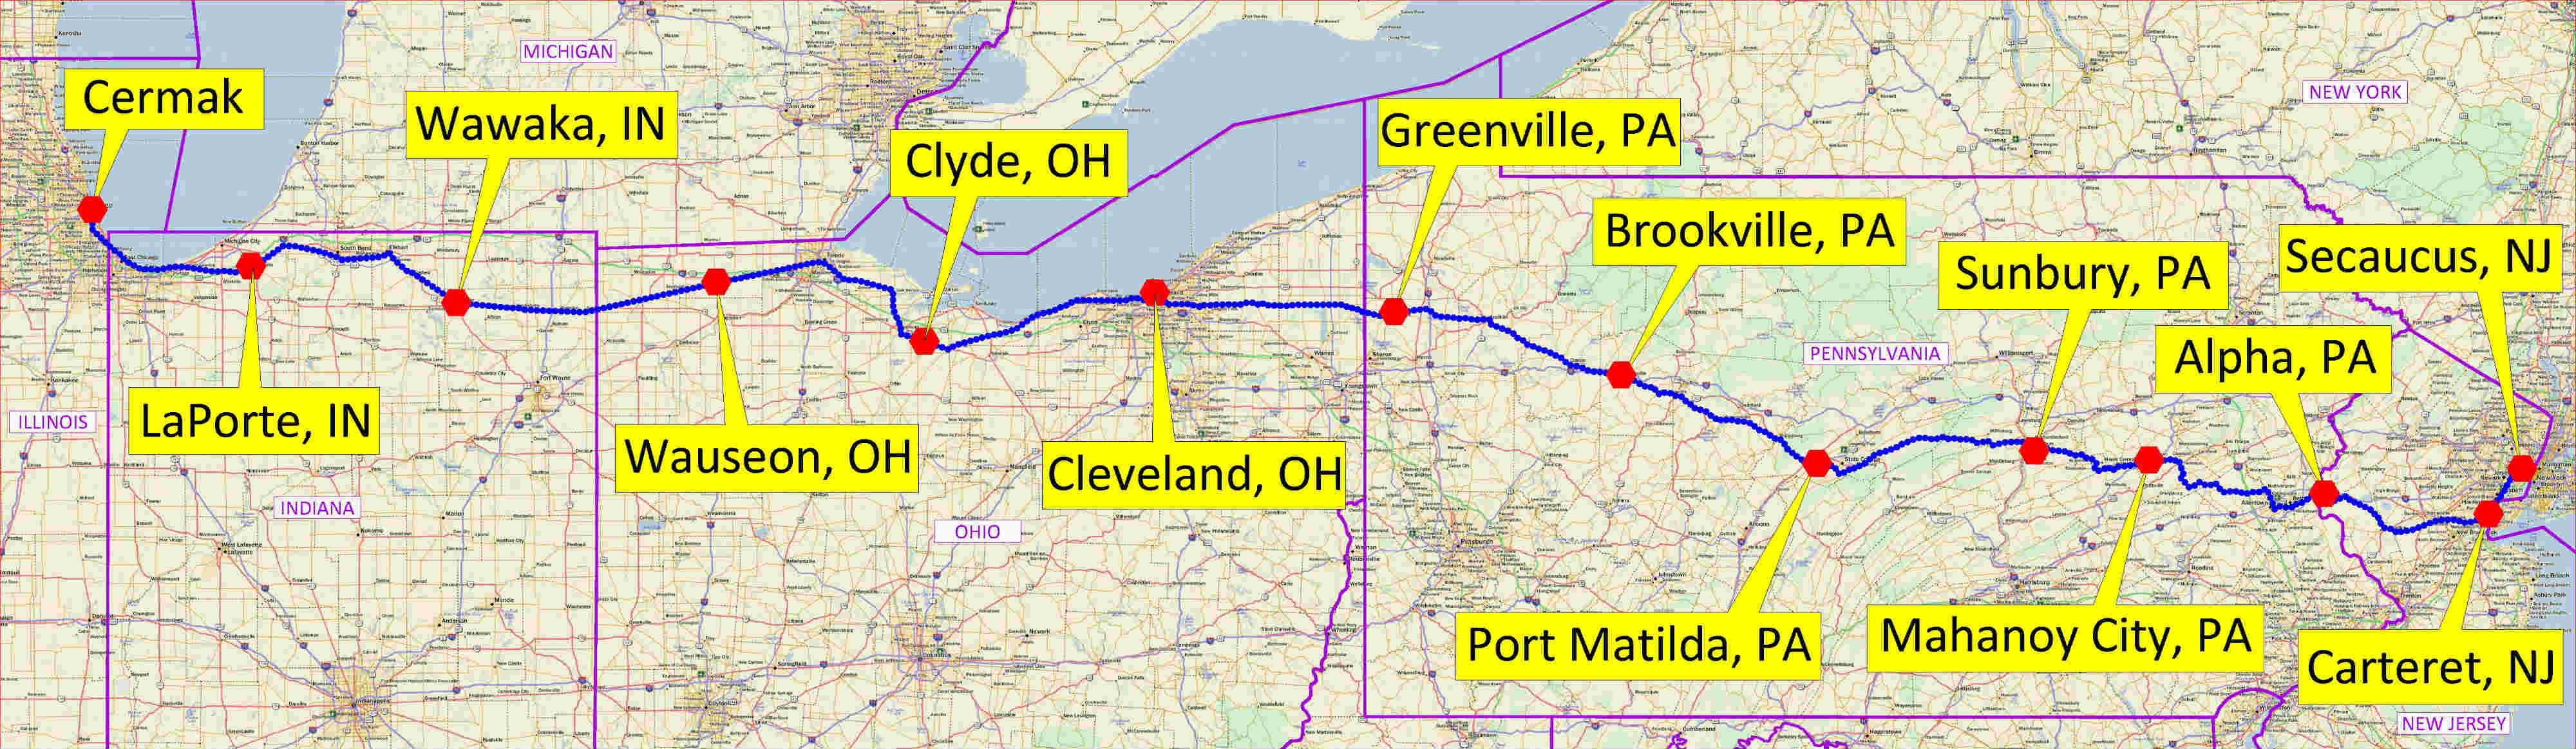
\includegraphics[scale=0.08]{assets/map.jpg}

2012: McKay Brothers installs an overground microwave tower relay (these can be subject to degradation in poor weather conditions)

2017: Go West consortium consolidates fiber optic, microwave, and undersea cables between Chicago and Tokyo

Some more speculative technologies include bouncing shortwave radio off the ionosphere for transoceanic communication, and use of inter-satellite laser links to travel through a vacuum instead of air.

\subsubsection{Physical Media}
Latency is either along the cable or on one of the ends.

The longer the distance, the more we care about effects that scale linearly with distance.

For private WAN links, we care mostly about the \textbf{propagation delay} of the medium, and the overhead required to remedy \textbf{attenuation}.

Here's the main diagram from Arista's \textit{Copper is Faster than Fiber}:
\begin{center}
	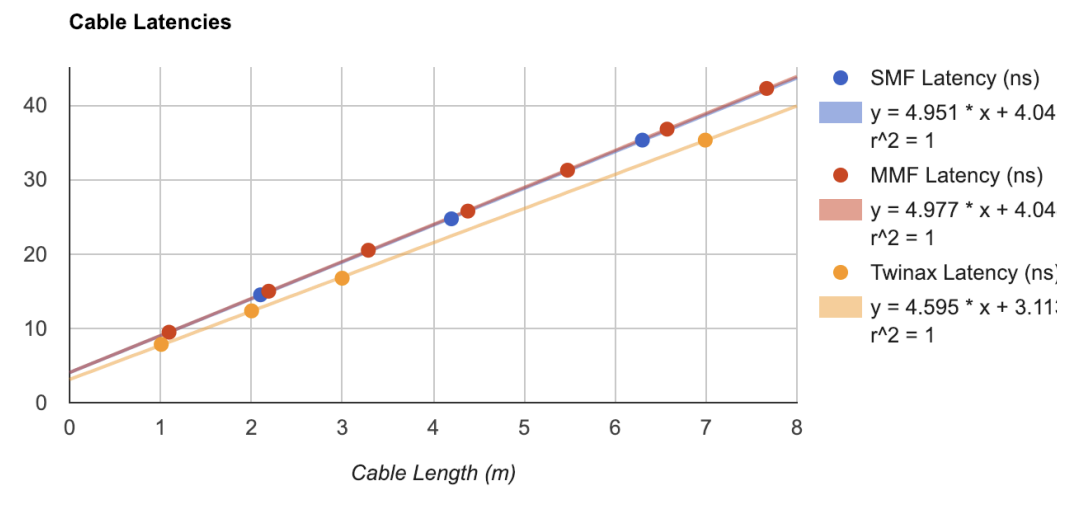
\includegraphics[scale=0.5]{assets/arista.png}
\end{center}
Despite higher propagation delay, fiber is used over copper for long distances because it has lower attenuation overhead.

\subsection{Colocation}
\subsubsection{Direct Market Access}
The ideal case is to be in the primary colocation. The next best thing would be proximity hosting. In the case of crypto, it helps to be in the same AWS regional data center.

Fairness is often a strong consideration for exchanges and regulators, especially when latency is very deterministic.

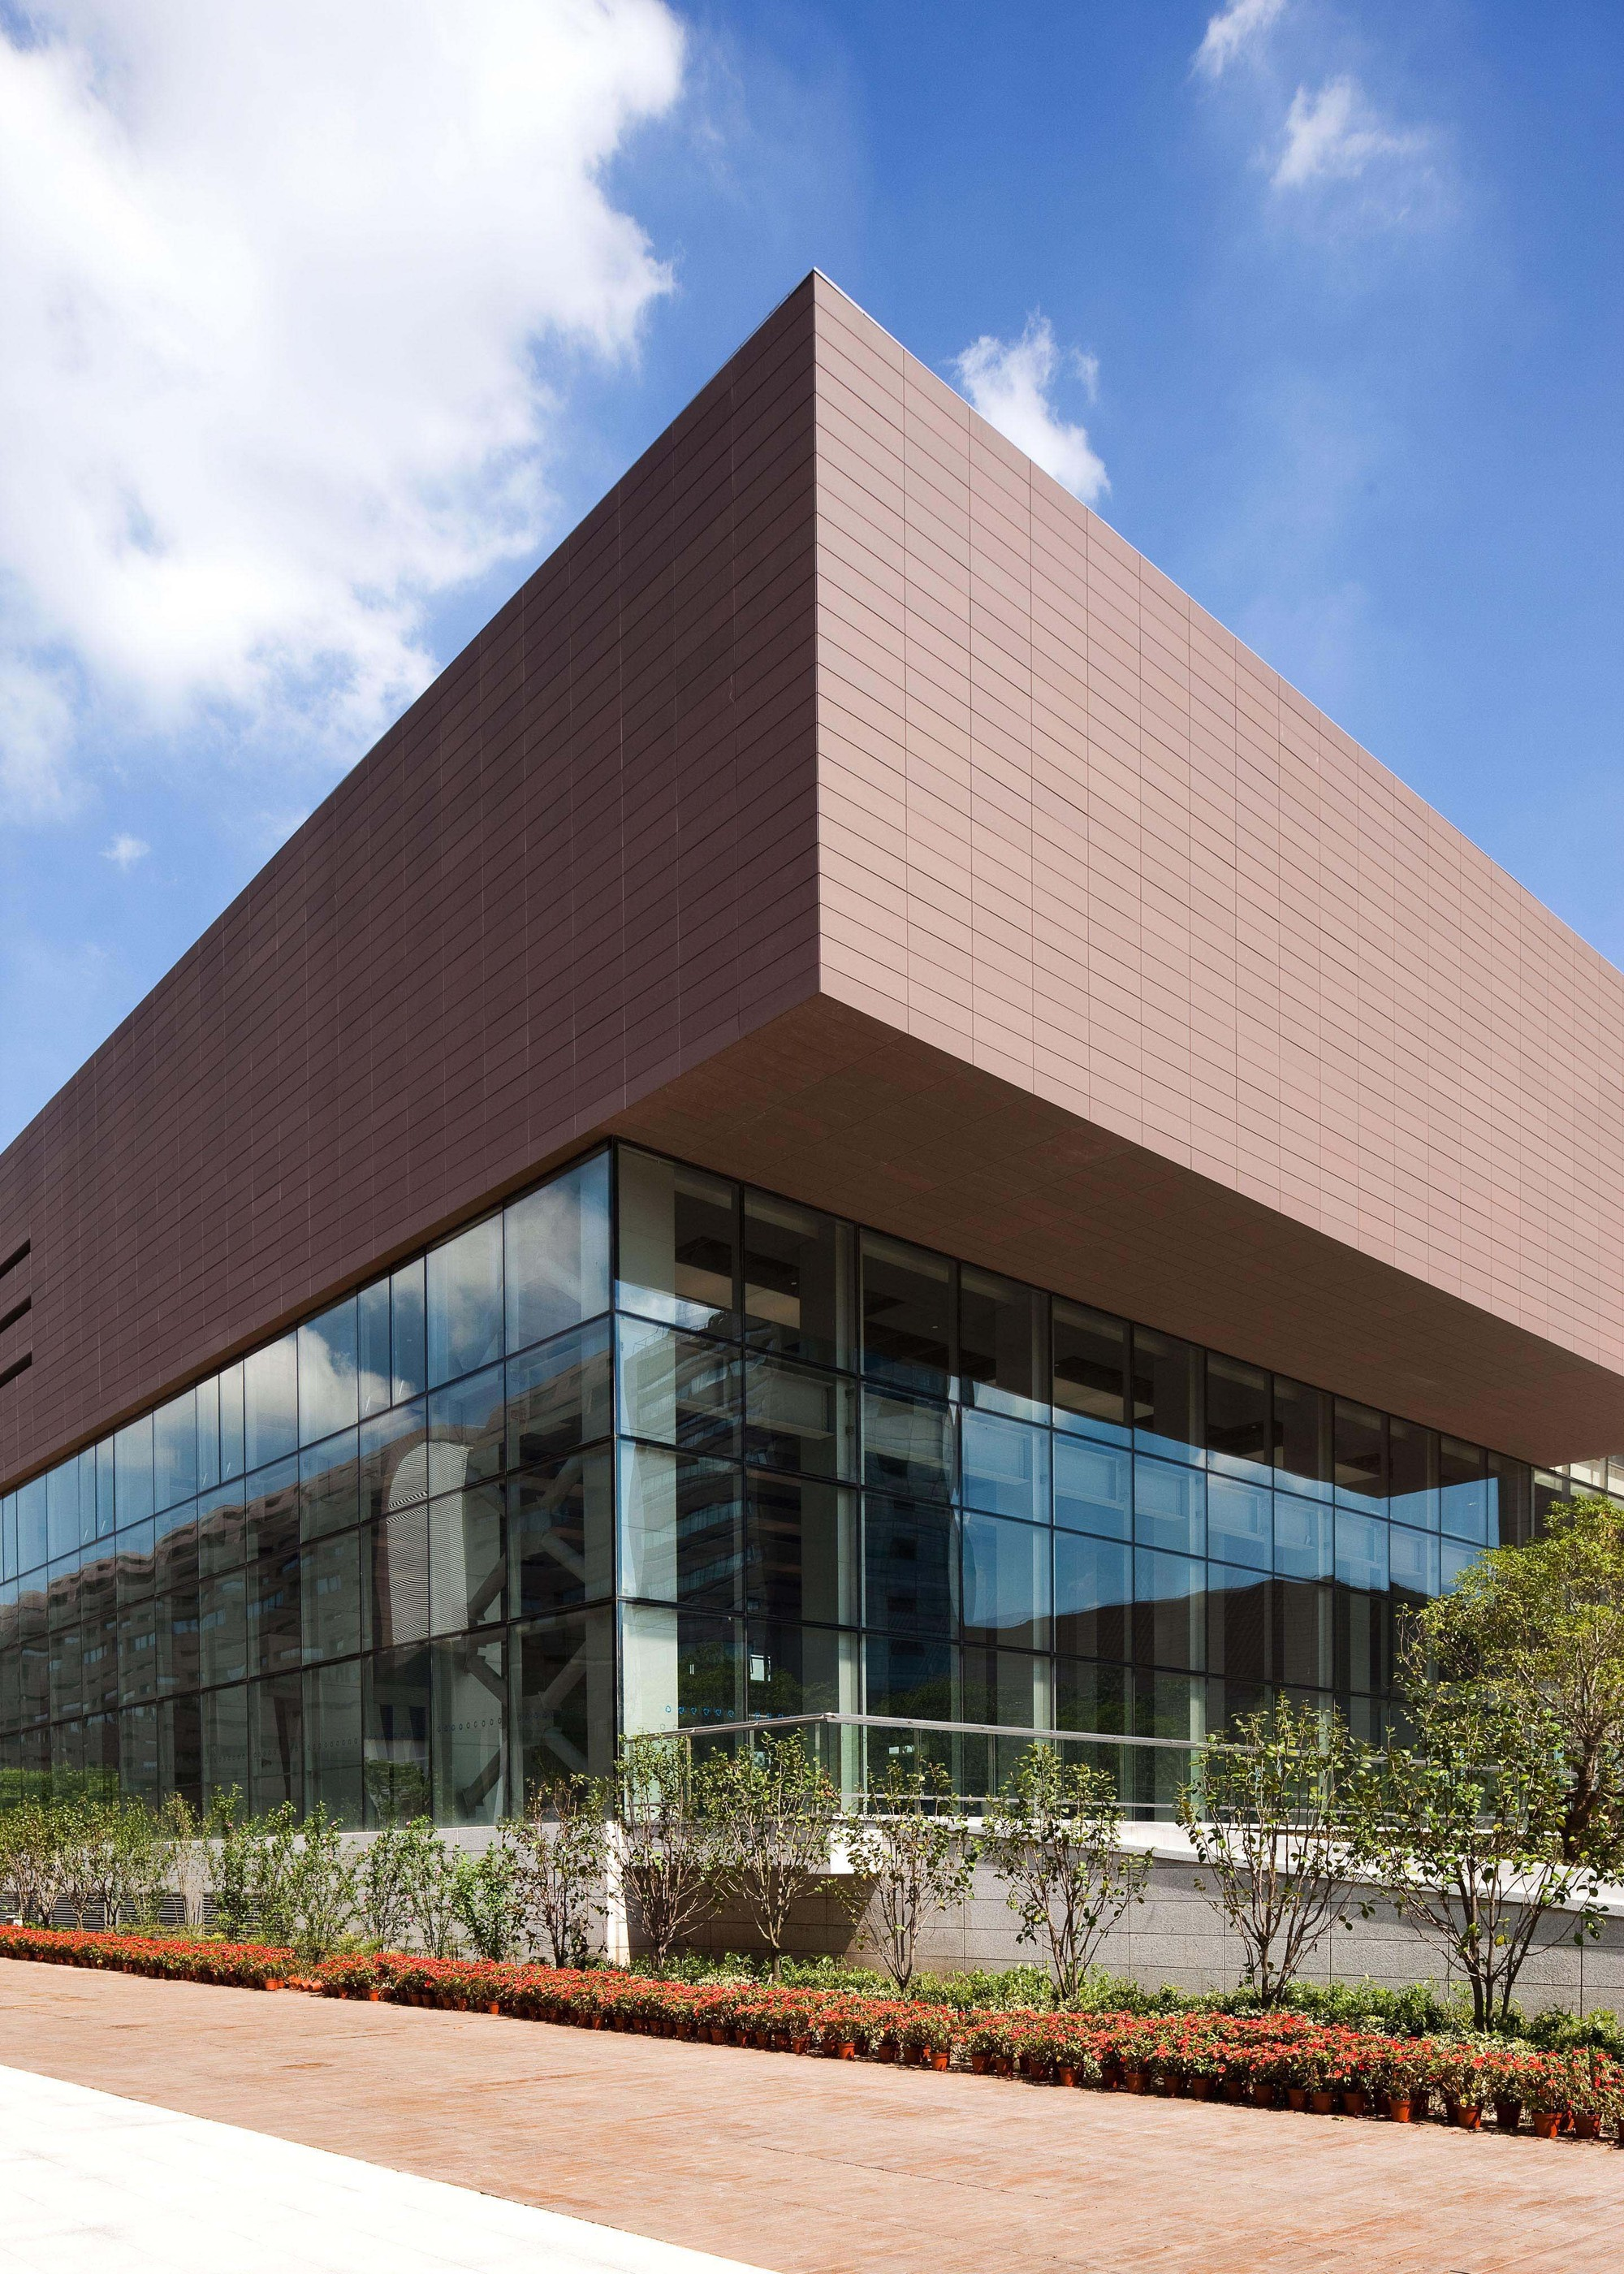
\includegraphics[scale=0.035]{assets/shfe.jpg}
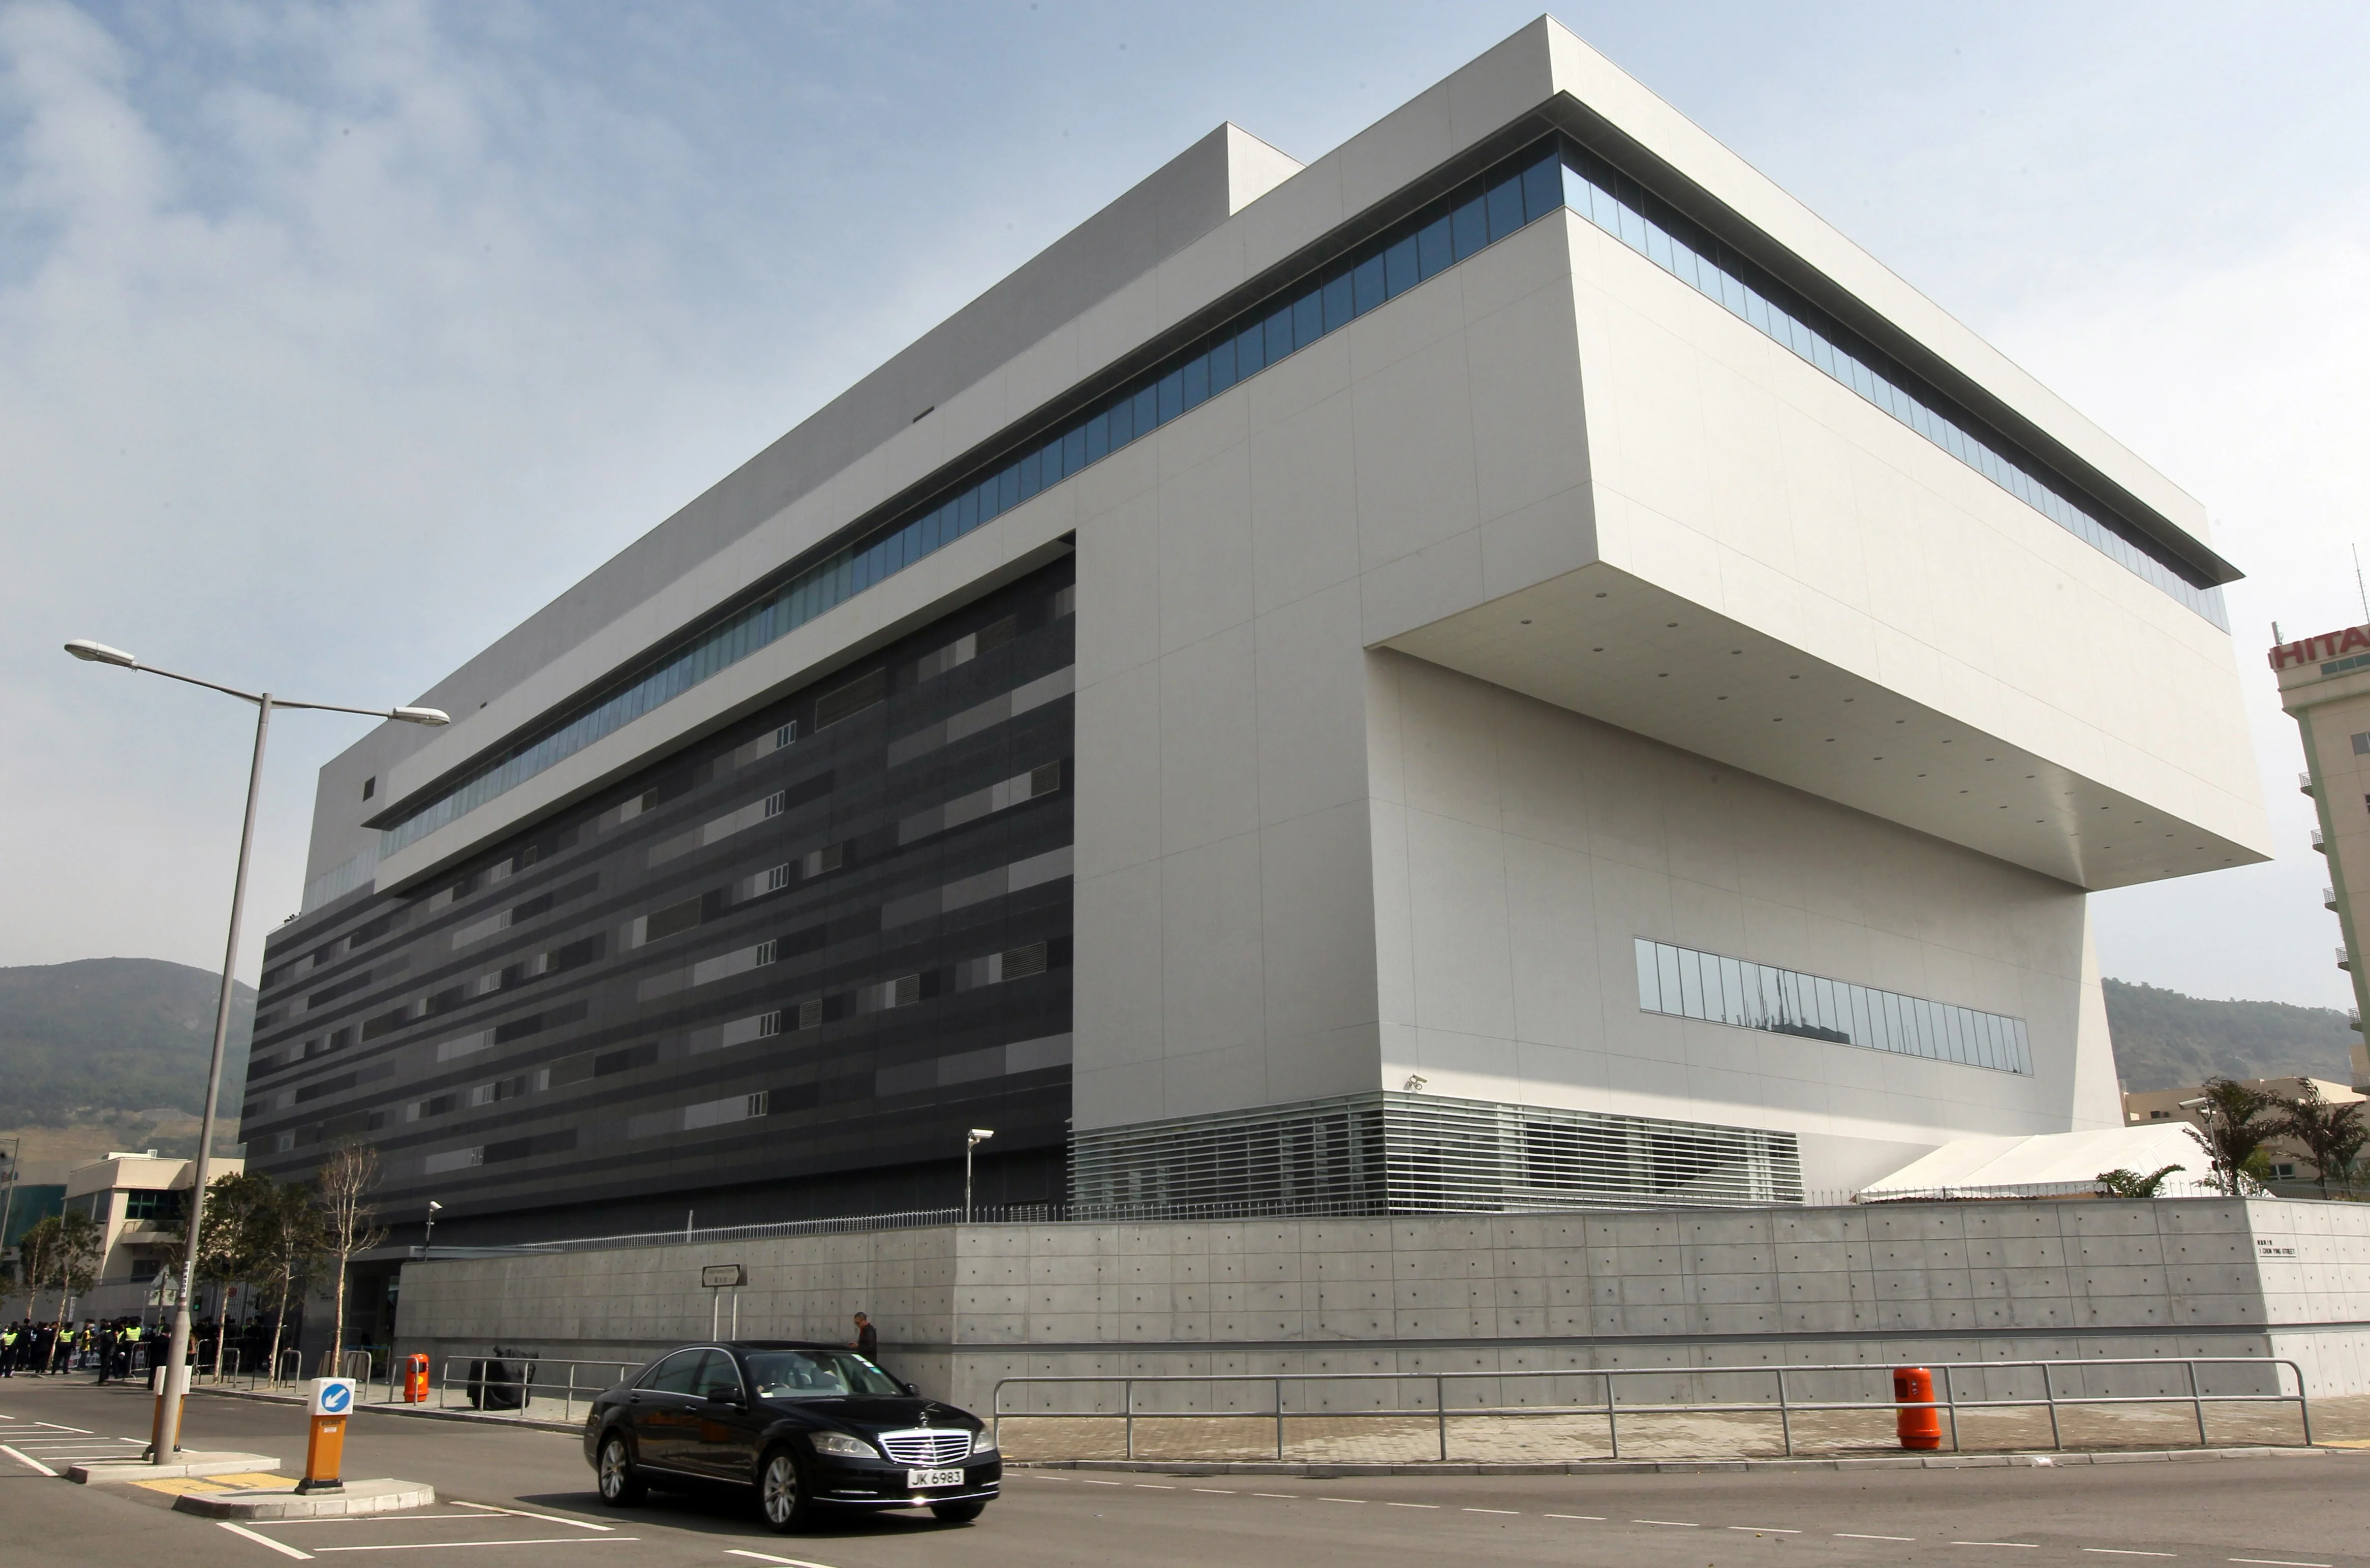
\includegraphics[scale=0.03]{assets/hkex.png}
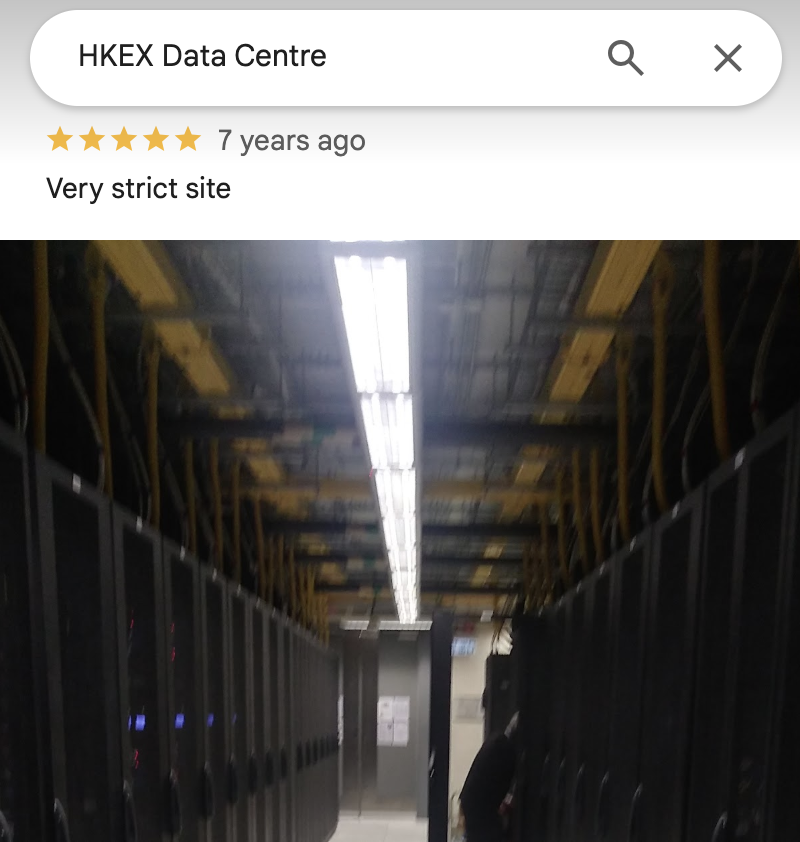
\includegraphics[scale=0.25]{assets/review.png}
\begin{block}{Jan 19 (Reuters)}
	``China's securities regulator has asked brokers to \textbf{remove client-dedicated servers from data centers in local exchanges}, a move that will deprive rapid-trading "flash boys" of an edge against other investors \ldots High-frequency traders in China have long used servers situated at data centers run by futures and stock exchanges and owned by brokers to execute trades as \textbf{the physical adjacency shaves off milliseconds or even microseconds}.''
\end{block}

\sectionquote{``This new form of communication could have some utility.'' Guglielmo Marconi}
\section{Networking}
\begin{center} 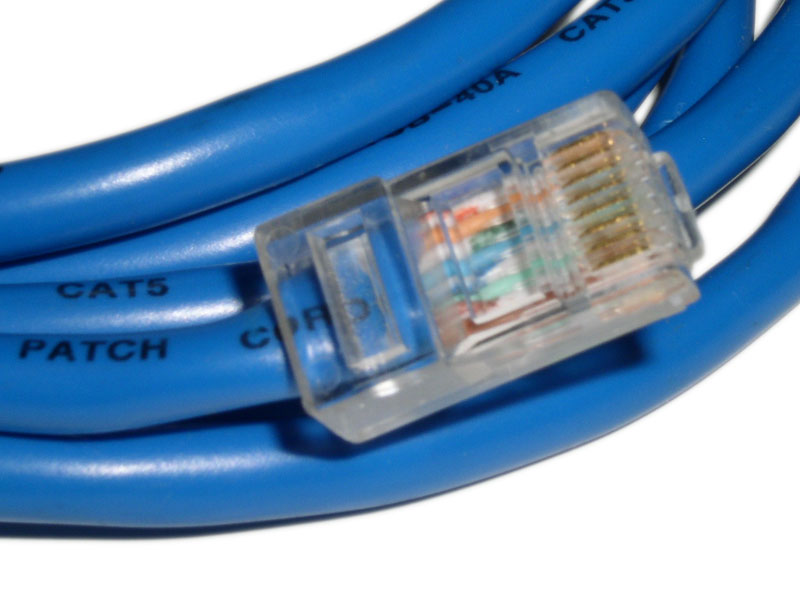
\includegraphics[scale=0.15]{assets/cat5.jpg} 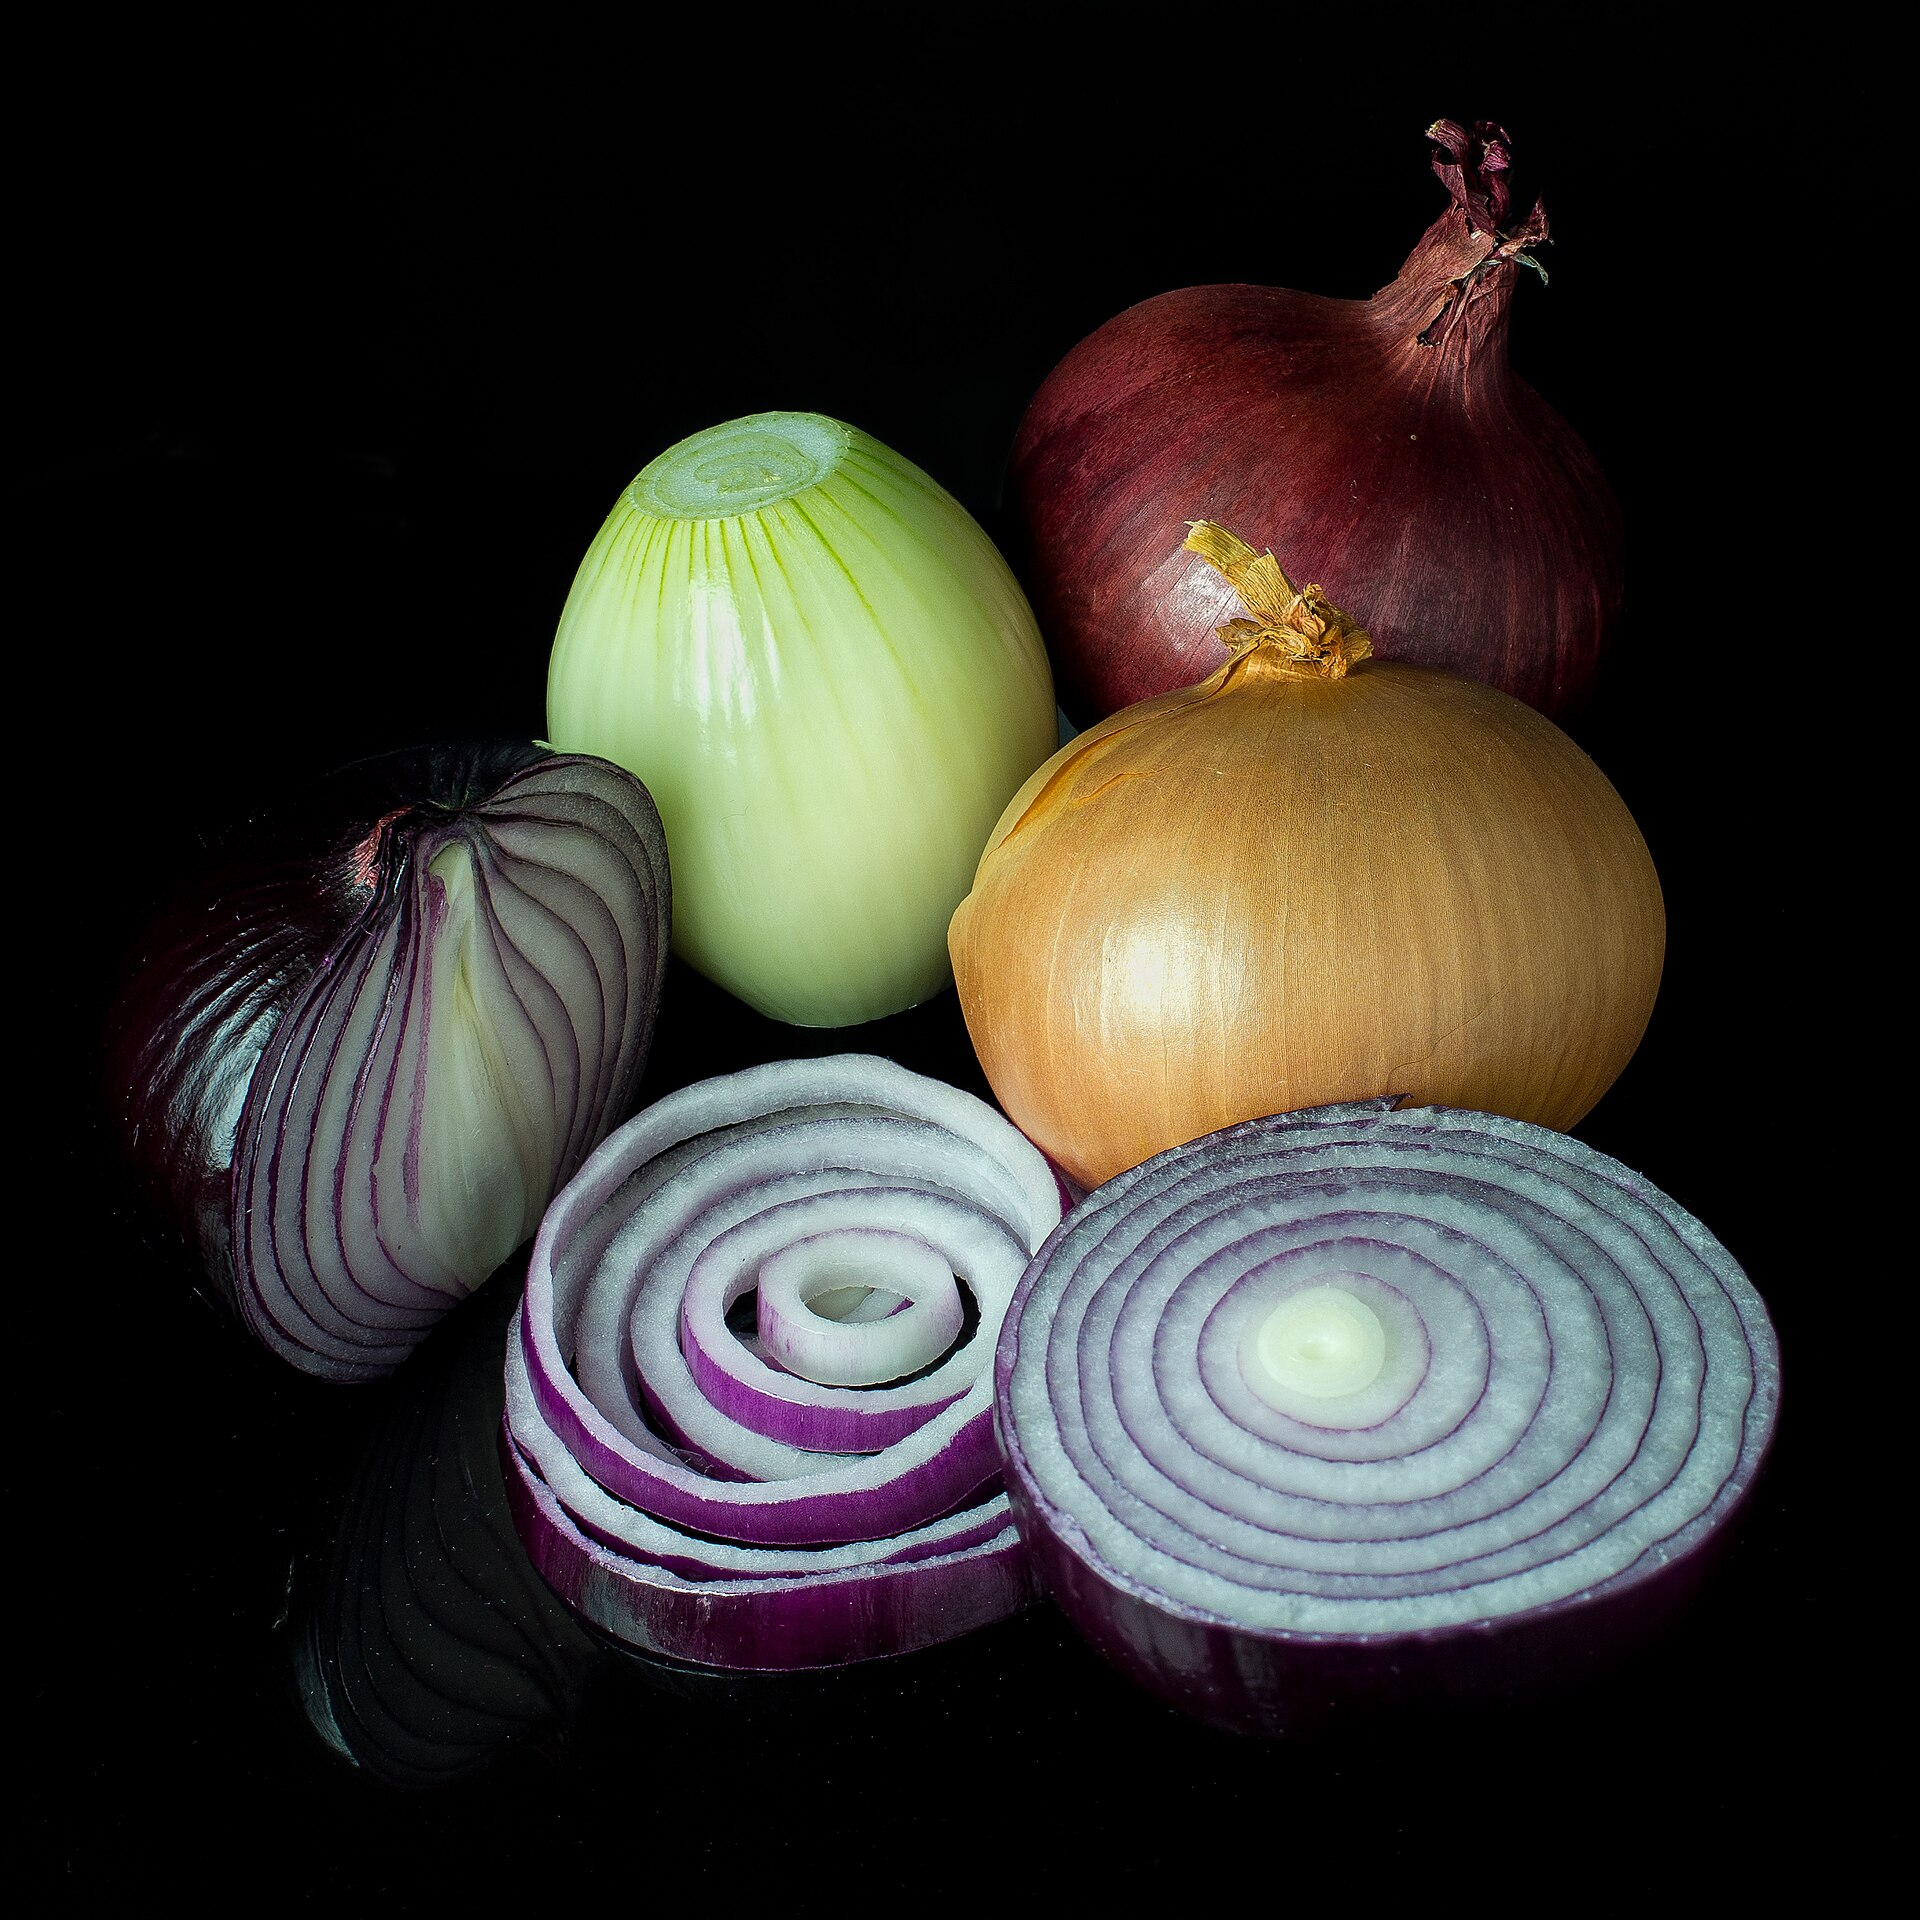
\includegraphics[scale=0.04]{assets/onion.jpg} \end{center}
\subsection{Networking Stack}
We will talk mainly about the first four OSI layers: physical (L1), ethernet (L2), IP (L3), TCP/UDP (L4).
\begin{center}
	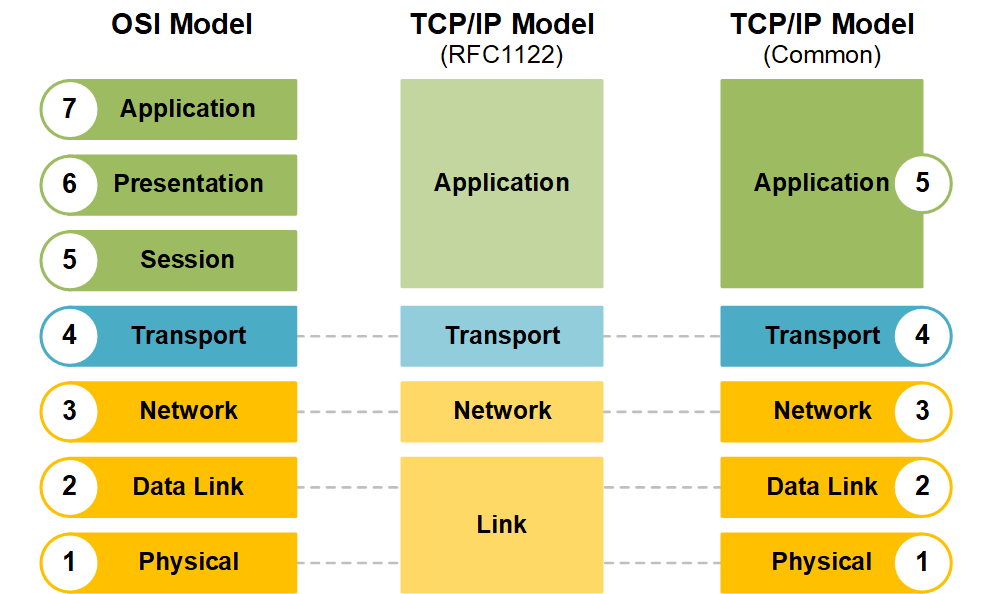
\includegraphics[scale=0.6]{assets/osi.png}
\end{center}

\subsubsection{Hardware}
\begin{itemize}
	\item 1969: NPL network becomes operational, governed by a central `routing' computer rather than an L1 crosspoint
	\item 1977: Patent granted for Ethernet, introducing CSMA/CD
	\item 1986: AT\&T develops StarLAN, one of the first topologies to use Ethernet hubs.
	\item 1986: DEC introduces the LANBridge 100 with a software-level MAC table and selective casting.
	\item 1989: Kalpana introduces EtherSwitch with a hardware-level MAC table, allowing half-duplex cut-through switching
	\item 1995: Cisco releases the Catalyst 5000 switch, supporting multicast switching
	\item 1999: Cisco releases the Catalyst 6000 switch, supporting Pulse Amplitude Modulation
\end{itemize}

Progress in networking has been largely dictated by commercial requirements different to those of HFT. Some of the older technologies that are no longer standard still see use in HFT.

\subsubsection{L2: Ethernet}
We send bits down the wire with some line coding and possibly modulation (L1).

The preamble tells the receiver the phase/frequency of the signal. Following the SFD, we identify the recipient \& sender, include some payload (up to 1500 bytes, ignoring nonstandard `jumbo frames'), and end with a checksum. We also have to wait 12 bytes between frames.
\begin{center}
	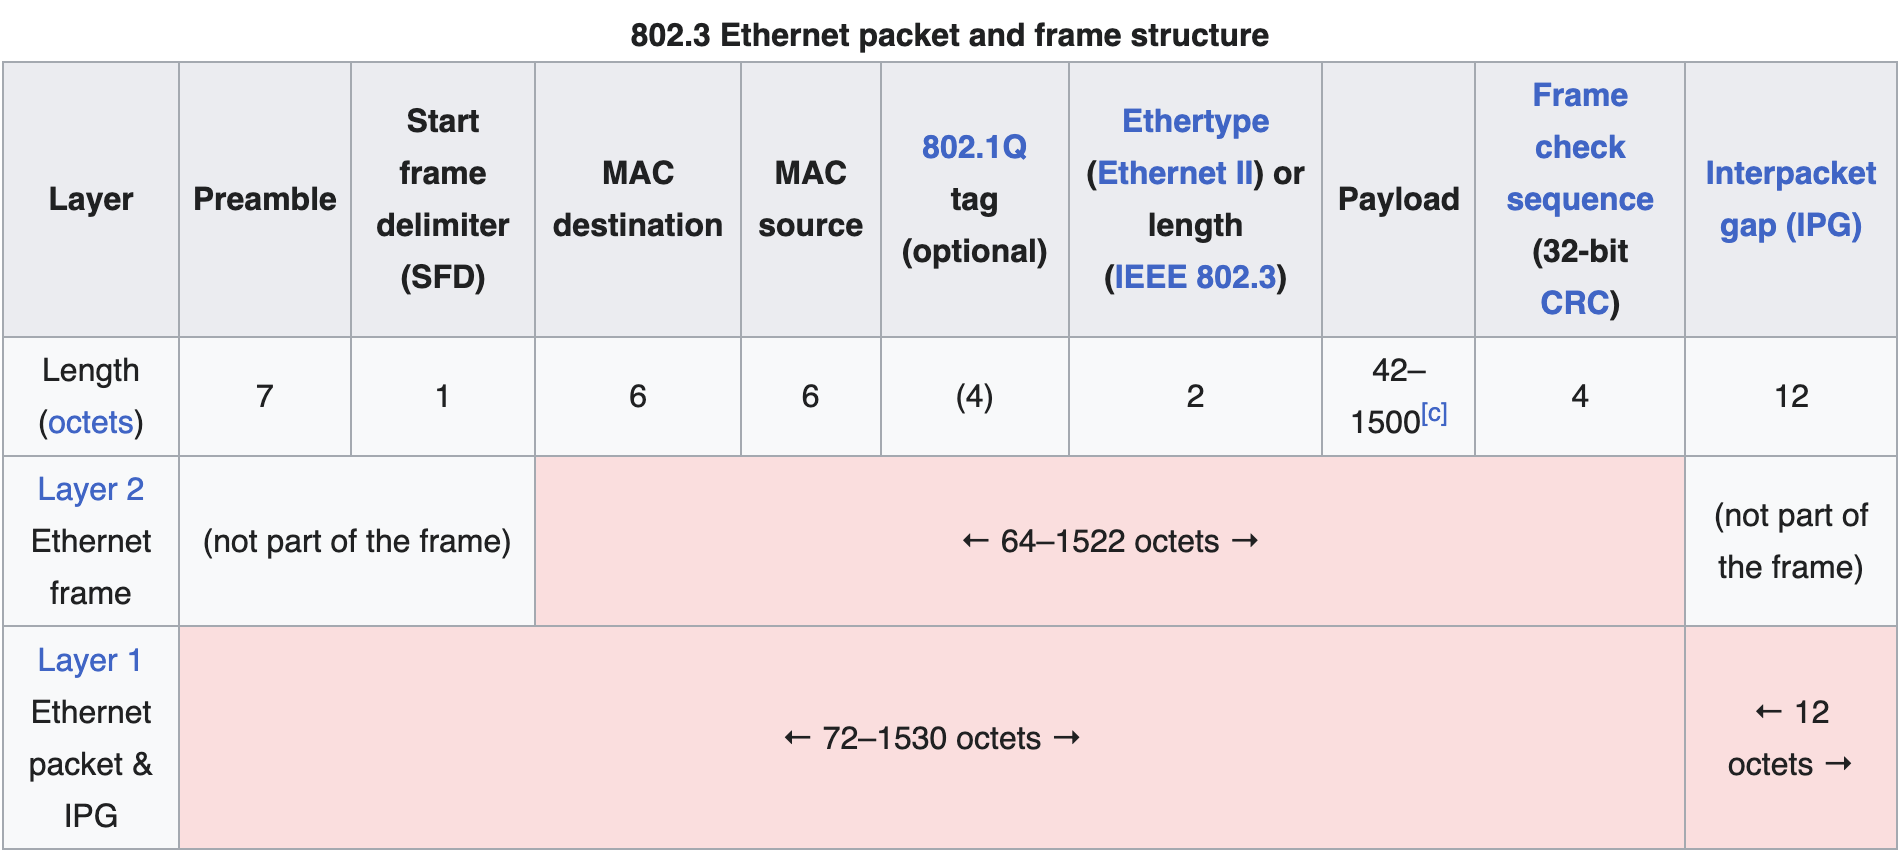
\includegraphics[scale=0.37]{assets/ethernet.png}
\end{center}
MAC addresses can indicate a single device, multicast group, or broadcast message. Since they are fixed at time of manufacture they can be used to identify the make of a device.

\subsubsection{L3: IP(v4)}
For typical use cases the ethernet payload starts with the IP header. This serves a similar purpose but also supports internetworking.
\begin{center}
	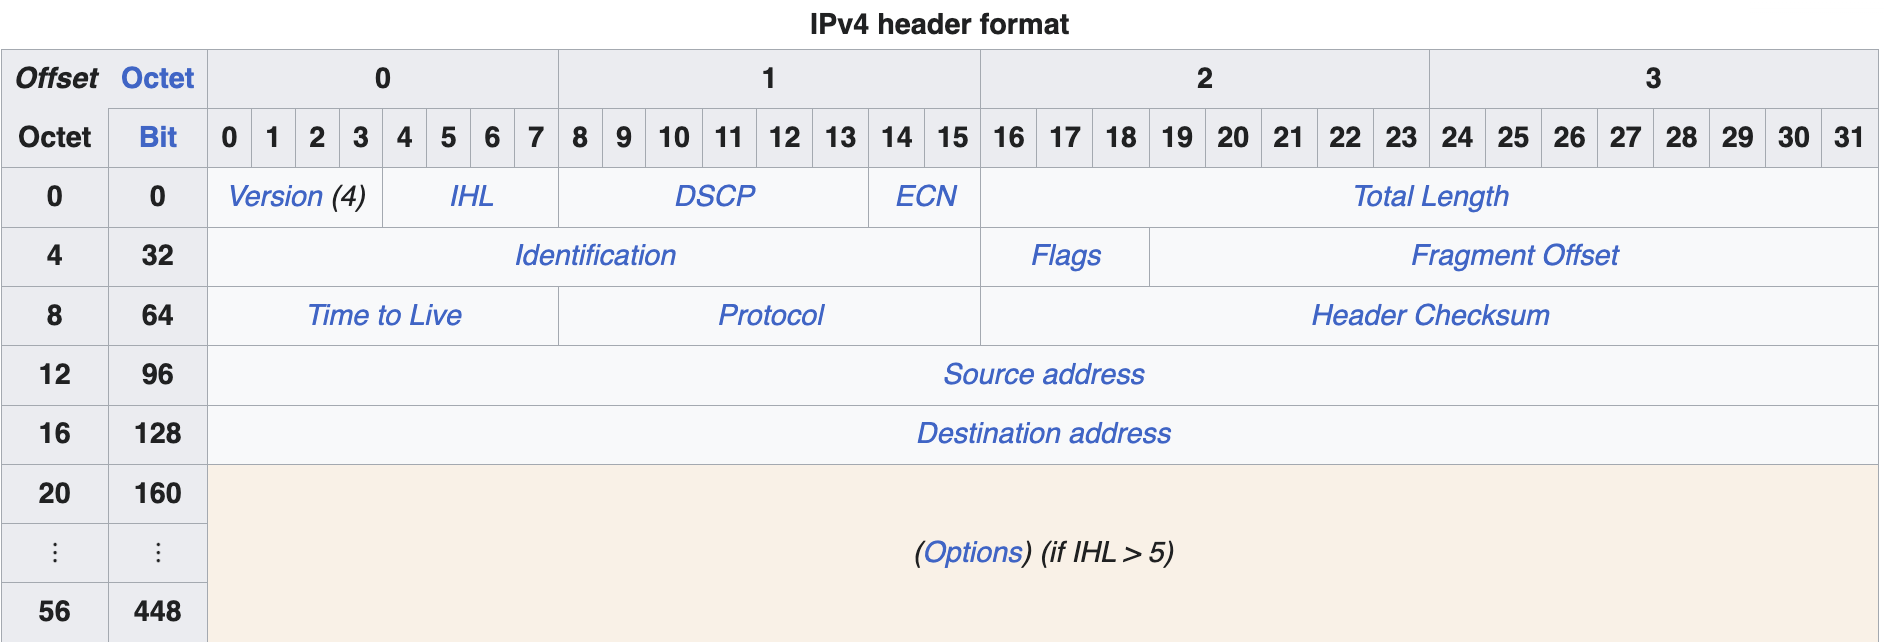
\includegraphics[scale=0.37]{assets/ipv4.png}
\end{center}

\subsubsection{L4: UDP}
The ports are numbers between 0-65535. They typically indicate what application-layer protocol is being used. These work the same way for TCP.

We also get the length in advance.
\begin{center}
	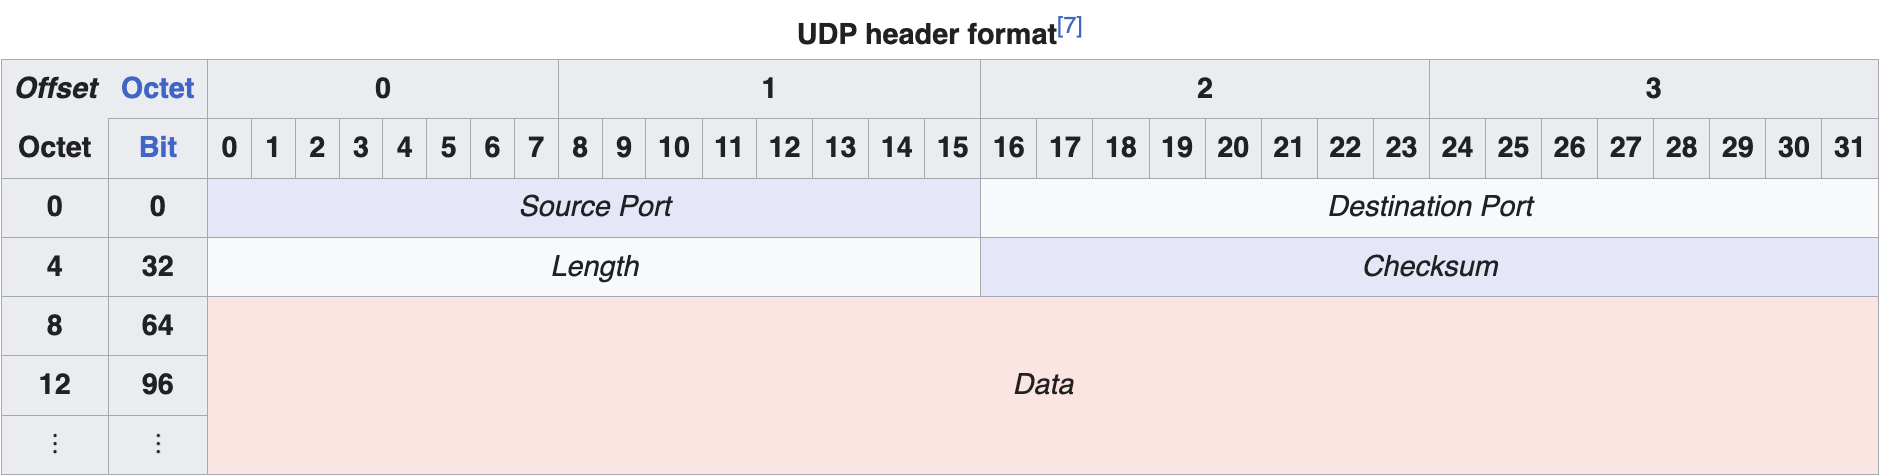
\includegraphics[scale=0.37]{assets/udp.png}
\end{center}

\subsubsection{L4: TCP}
TCP uses sequence numbers and the ACK field to recover from the case where data is dropped.
\begin{center}
	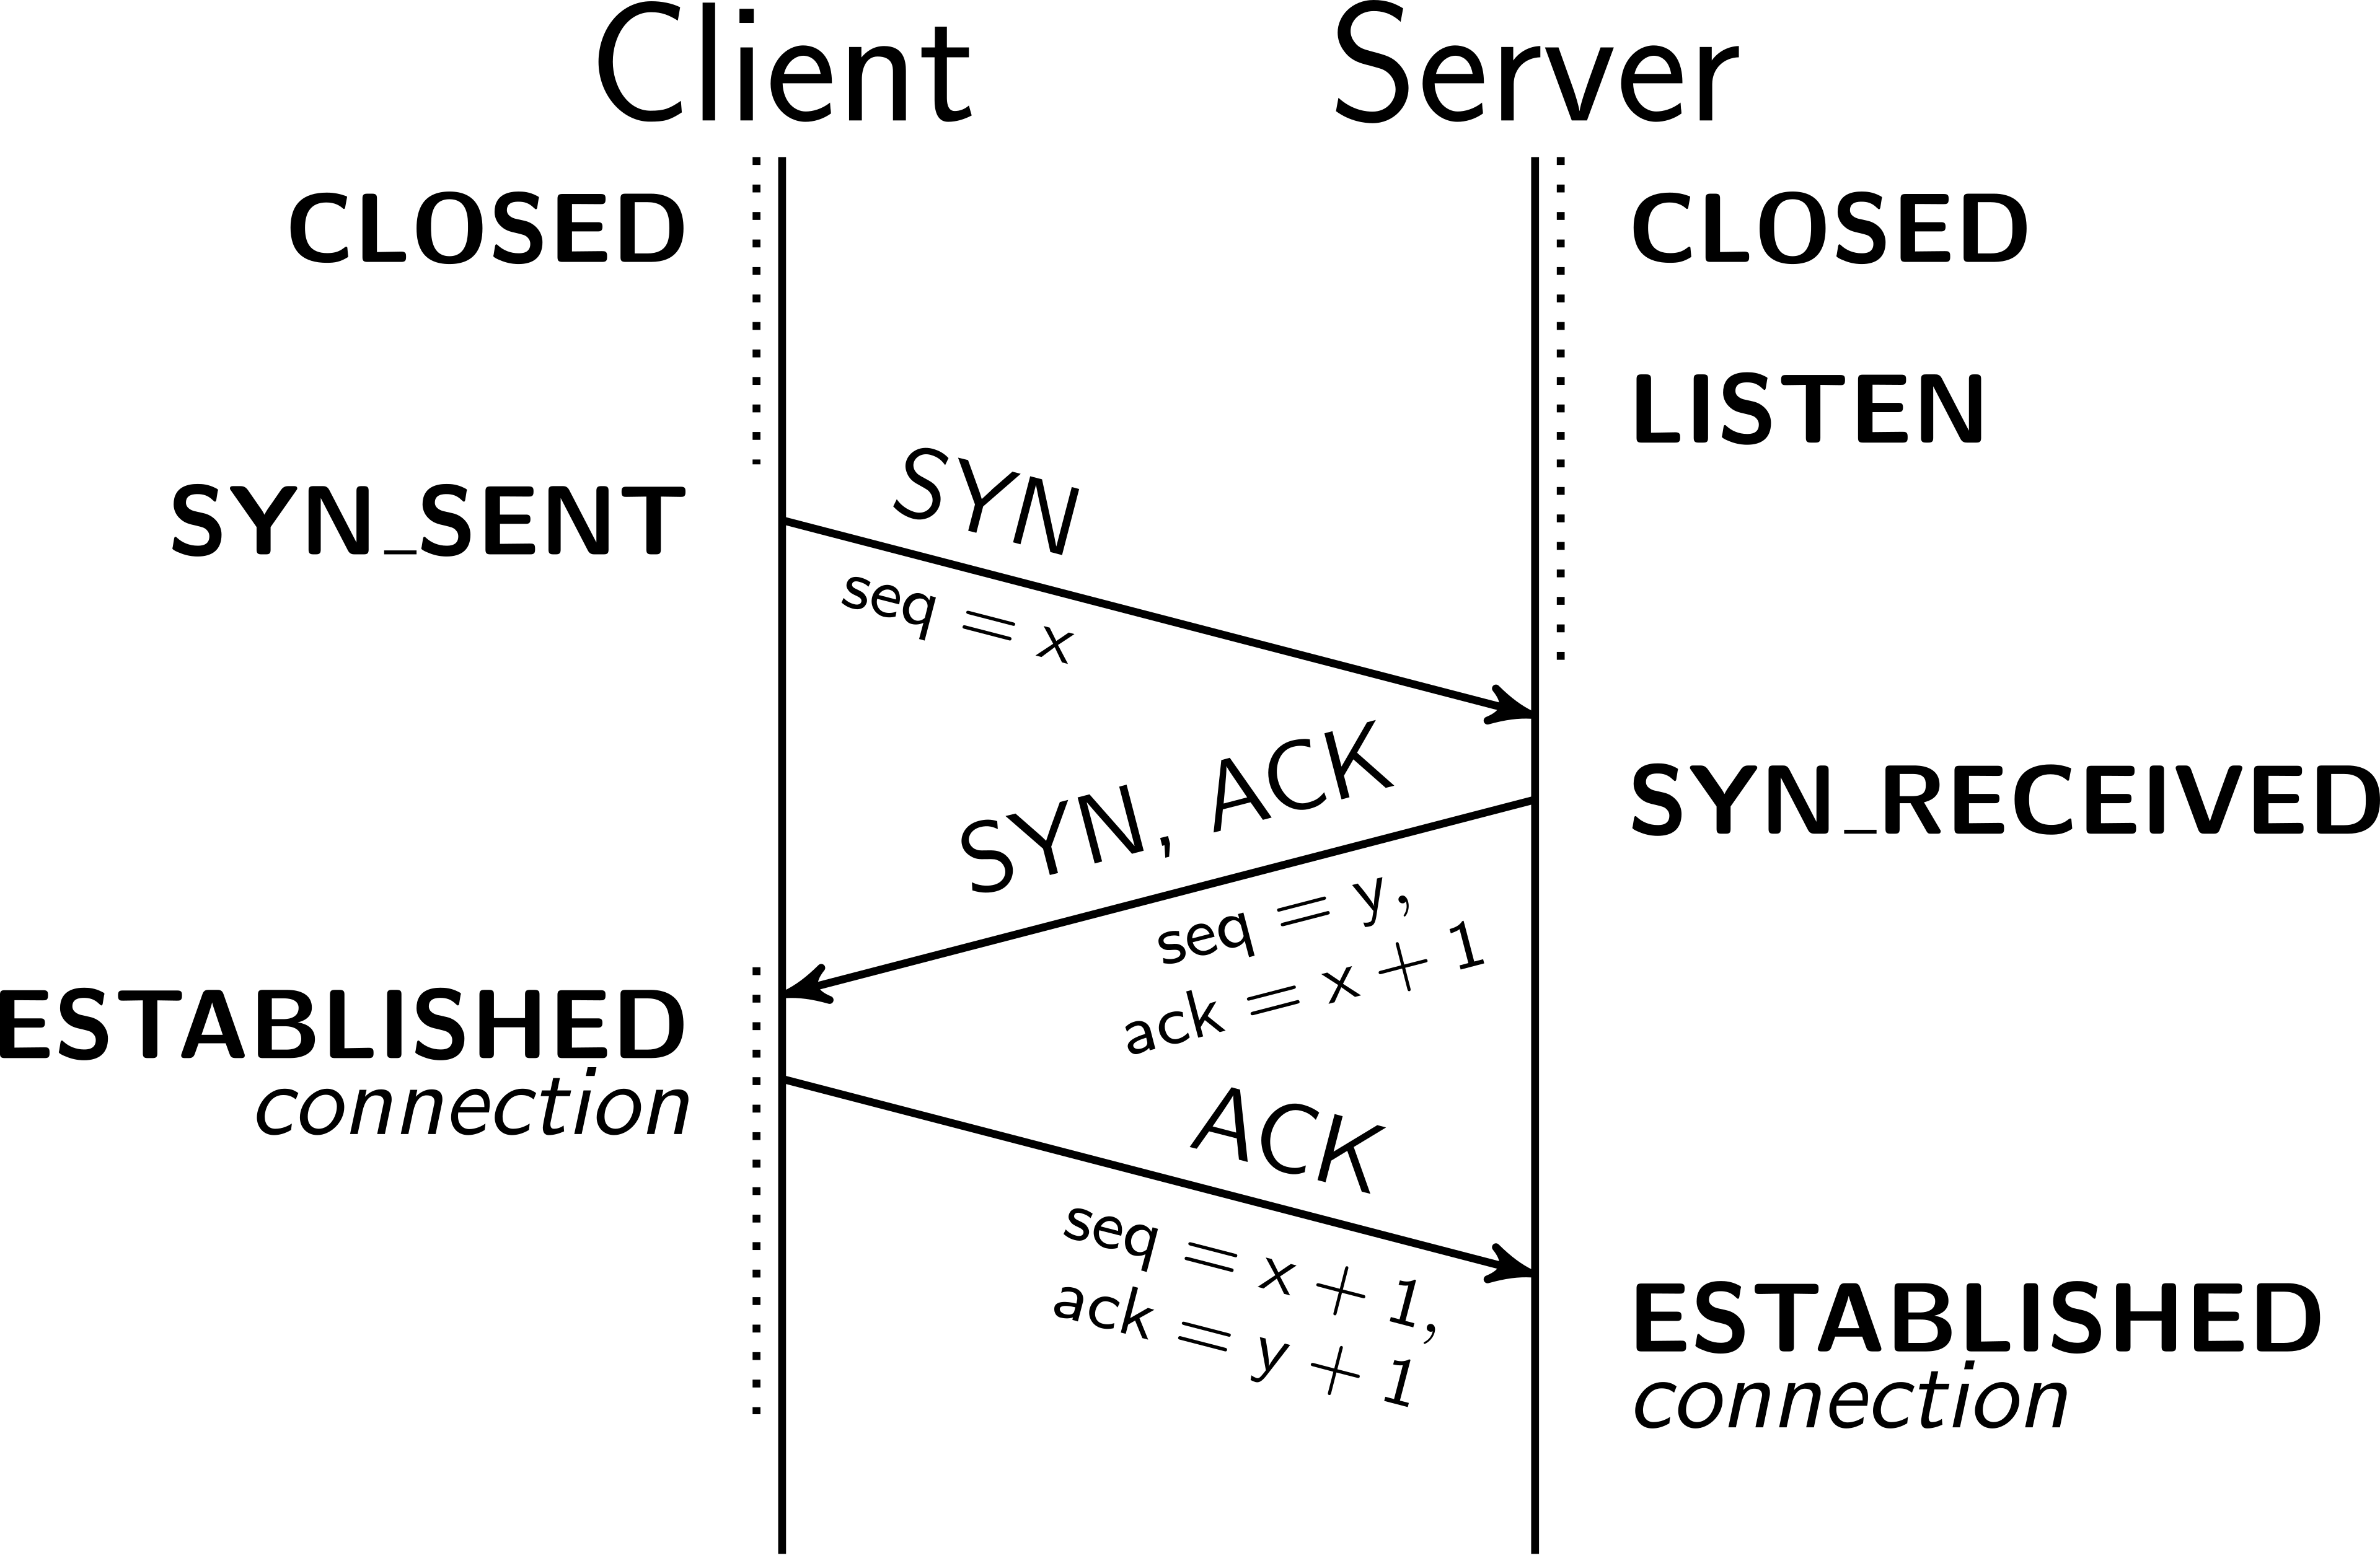
\includegraphics[scale=0.08]{assets/handshake.png}
\end{center}

\begin{center}
	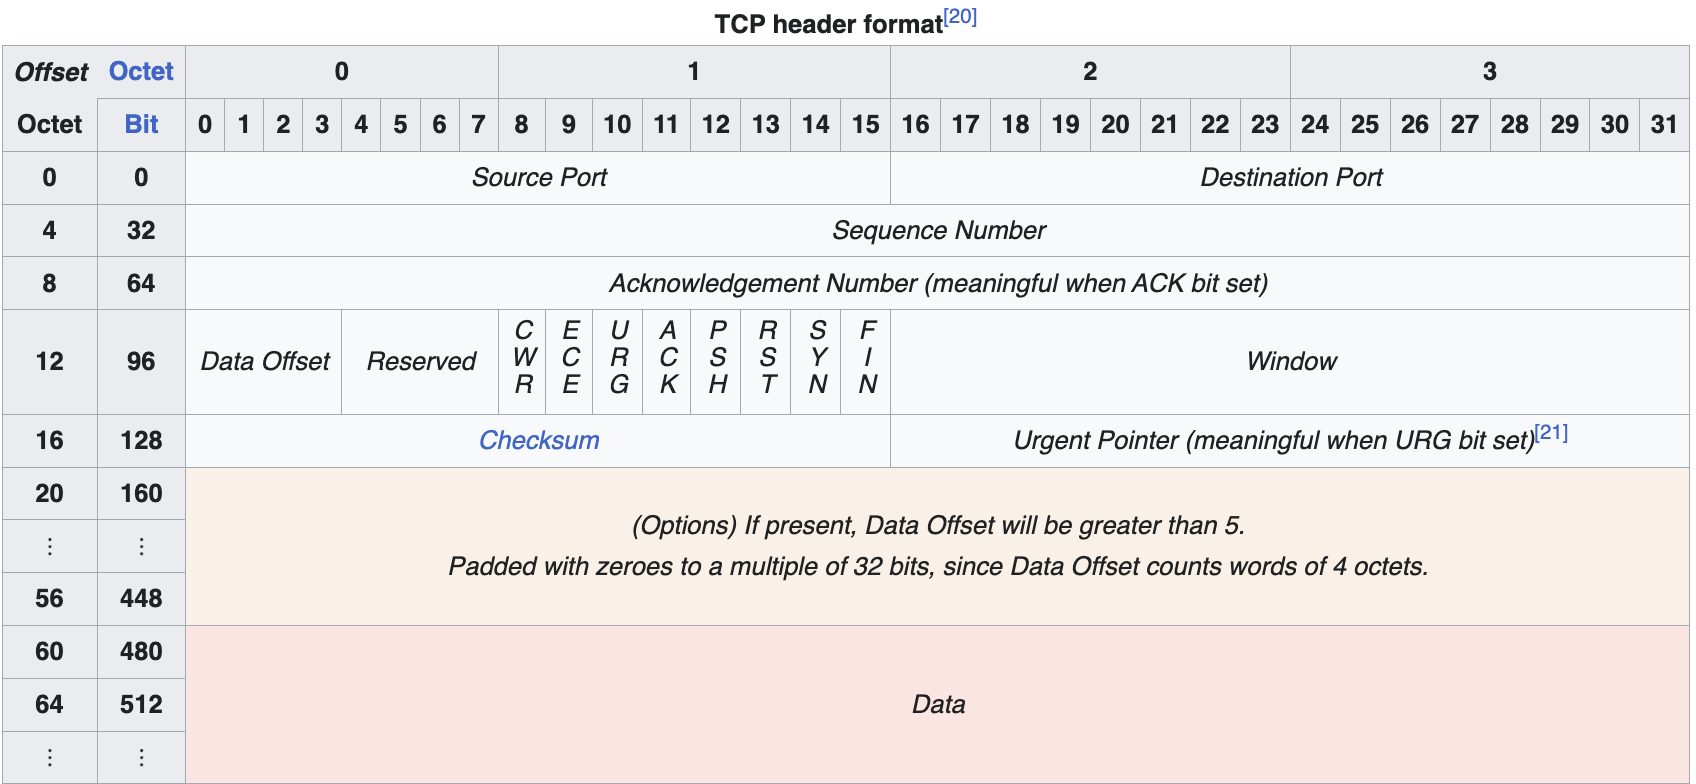
\includegraphics[scale=0.4]{assets/tcp.png}
\end{center}

In the recording I give a very quick demo of Wireshark for parsing L1-L4.

\subsection{Common Exchange Protocols}
\href{https://www.nasdaqtrader.com/content/technicalsupport/specifications/TradingProducts/OUCH5.0.pdf}{OUCH} (Execution) and \href{https://www.nasdaqtrader.com/content/technicalsupport/specifications/dataproducts/NQTVITCHSpecification.pdf}{ITCH} (Market Data) are common for Nasdaq-designed systems.

\href{https://fixtrading.org/packages/fix-tagvalue-encoding/}{FIX} is a more general purpose ASCII-encoding.

\subsection{Network Timestamping}
Timestamping of messages may be done at multiple points in the system (e.g. \texttt{timestamp\_match} and \texttt{timestamp\_publication}).

Timestamps from different clocks (e.g. from different machines) are not trivial to compare owing to \textbf{clock drift} and \textbf{clock sync inaccuracies} (e.g. caused by network asymmetry).

Usually the timestamp is calculated according to the first bit of the Ethernet header (start-of-frame). The last bit timestamp can be inferred using the bandwidth of the transmission.

\subsection{Local Network Topology}
\subsection{Abstract Colocation Topology}
\diagram{}

\subsection{Example Colocation Topology}
\begin{center}
	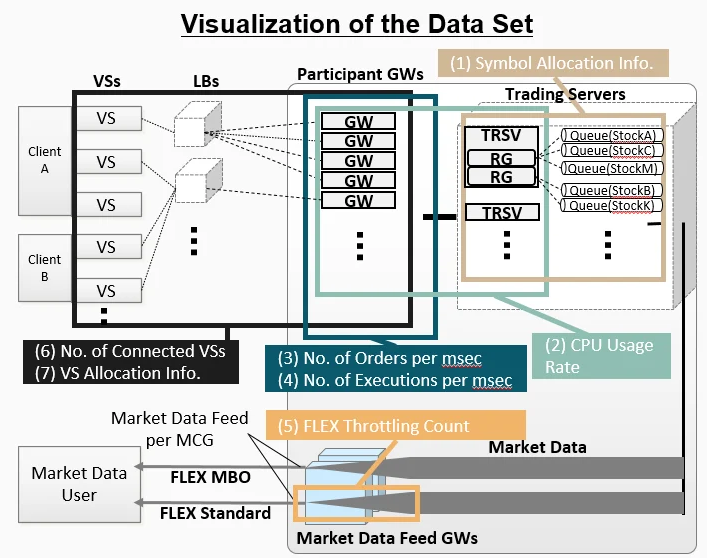
\includegraphics[scale=0.4]{assets/tse.png}
\end{center}
Exchange documentation is a starting point but cannot always be fully trusted.

\part{Network Latency}

\sectiondiagram{execution}
\sectionquote{``We affirm that the world's magnificence has been enriched by a new beauty: \\the beauty of speed.'' Filippo Marinetti}
\section{Execution}

\subsection{Compliance}
\subsubsection{Externalities}
\begin{block}{}
	``What if you want to be a bit more unpleasant? How about you work out \ldots \textbf{which is the best gateway to connect to?} \ldots You can start sending your orders through that.

	What about all these \textbf{other gateways}? What if you start stuffing orders through those other gateways that you don't care for matching? \ldots They're now \textbf{stuffed up with traffic} so other people can't compete.

	Then you go through the gateway that you have set up which you know is fast, and you're going to send your orders through nice and quick.'' Martin Thompson, \href{https://www.infoq.com/presentations/financial-exchange-architecture/}{\textit{Evolution of Financial Exchange Architecture}}
\end{block}

If we're sending multiple copies of the same order we might want to ensure idempotency somehow. Otherwise we will need to consider the possibility that we get more than one fill.

Because people often behave themselves and it is not so easy to tell when they don't, a lot of these regulations are never tested. The politically incorrect way to put this would be that `compliance' is better thought of as a spectrum of more or less commercially viable behaviours.

\textbf{Load balancers} help accommodate the large volume of data moving through the network, particularly during significant market events.

\subsubsection{Compliance}
\begin{block}{Exchange Circular}
	``In order to ensure every EP can trade in a fair and orderly market, activities including the following \ldots are therefore prohibited:
	\begin{enumerate}
	\item Deliberate fragmentation of Transmission Control Protocol (TCP) messages (‘packet splitting’);
	\item Deliberate retransmission of TCP or application layer messages;
	\item Deliberate transmission of corrupt network packets;
	\item Inappropriate/excessive use of non-trading messages such as heartbeat, connection management; and
	\item Hold up or interfere with normal queuing and processing of network or application messages.''
	\end{enumerate}
\end{block}

\subsubsection{Fragmentation}
TCP/UDP Protocol Data Units (PDUs) can be split across multiple Ethernet frames. The recipient will hold these fragments for some time waiting for the rest of the PDU, then discard them.

\begin{block}{}
	``The virtual channels on the X.25 for ordering were only 64kbps – very slow. I figured we could hack those similarly \ldots and start filling out an order before we had one. This would save us milliseconds. You could turn the packet into something benign or invalid if you didn’t have an order.'' Matt Hurd
\end{block}

Some overhead is added by the Ethernet preamble/FCS/IPG when fragmenting. This shouldn't matter if the fragments are sent very far apart.

Exchanges typically monitor packet corruption rates for signs of abuse.

\paragraph{Quantifying Speedup}

So long as everything fits within 1500 bytes and the later frame does not queue behind the pre-sent frame:
\begin{itemize}
	\item This will have no effect on first-bit latency for a cut-through switch.
	\item For a store-and-forward switch, it will save time equal to the number of bits present divided by the bandwidth.
\end{itemize}

If our total message exceeds 1500 bytes then we would need to consider whether this changes the number of frames we need to send when the trade is triggered.

This is just the L1/L2 network latency. There may be other effects once the frame reaches the gateway.

\subsubsection{Deterrents}
\begin{block}{Exchange Circular}
	``An enhancement to the Market Segment Gateway (“MSGW”) will be introduced to further safeguard the \ldots electronic trading platform \ldots infrastructure by introducing a delay of at least three microseconds if the MSGW receives a partial order message as a means of ensuring the stability of the platform. Certain participants \textbf{intentionally submit partial order messages to reduce latency, and only complete the order message upon the happening of an event or trading signal.} Implementation of the enhancement is expected to reduce the frequency of intentionally split order messages as the additional processing time will serve as a deterrent.''
\end{block}

Exchanges often limit throughput (`\textbf{transactions per second}').

Limits might be per-session, per-user, etc.

\subsection{Out-of-Order Delivery}
Similarly, the use of sequence numbers in TCP makes it robust to out-of-order delivery of data:
\begin{block}{}
	``We were already sending the first part of the message in an early packet.

	Why not \textbf{send the later part of the packet} with the next TCP sequence number plus one \textbf{and then send the middle part of the sequence out of order} with the symbol, price and quantity?

	That final part of the packet had quite a large user field so we would save an awesome amount of time and gain much more than we were with the speculative send we were already doing.'' Matt Hurd
\end{block}

TCP guarantees delivery of a bytestream, and presentation-layer message boundaries need not align with packet boundaries. In practice they often do because events come in bursts.

\subsection{Win-rate Modeling}
Suppose all participants have independent latency with mean $\mu_i$ and a common standard deviation $\sigma$ (also called \textbf{jitter}).

If we model latency as a negative Gumbel distribution (normal-ish), the probability of being fastest is conveniently proportional to $\exp\left(\frac{\pi}{\sqrt{6}} \cdot \frac{-\mu_i}{\sigma}\right)$.

If every participant sends $n_i$ independent copies of their message, the probability of being fastest is proportional to $n_i \cdot \exp\left(\frac{\pi}{\sqrt{6}} \cdot \frac{-\mu_i}{\sigma}\right)$.

Of course, the latencies are usually not independent. With more specifics, we could build an explicit queueing model.
\begin{center}
	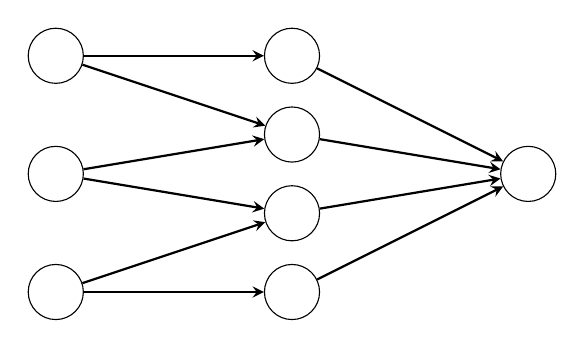
\begin{tikzpicture}[
	    >=stealth,
	    every node/.style={circle, draw, minimum size=7mm, inner sep=0pt},
	    arrow/.style={->, thick}
	]
		\node (a1) at (0, 1.5) {};
		\node (a2) at (0, 0) {};
		\node (a3) at (0,-1.5) {};

		\node (b1) at (3, 1.5) {};
		\node (b2) at (3, 0.5) {};
		\node (b3) at (3,-0.5) {};
		\node (b4) at (3,-1.5) {};

		\node (c1) at (6, 0) {};

		\draw[arrow] (a1) -- (b1);
		\draw[arrow] (a1) -- (b2);

		\draw[arrow] (a2) -- (b2);
		\draw[arrow] (a2) -- (b3);

		\draw[arrow] (a3) -- (b3);
		\draw[arrow] (a3) -- (b4);

		\draw[arrow] (b1) -- (c1);
		\draw[arrow] (b2) -- (c1);
		\draw[arrow] (b3) -- (c1);
		\draw[arrow] (b4) -- (c1);
	\end{tikzpicture}
\end{center}

\subsection{Lottery Game}
\begin{block}{}
	\begin{itemize}
	\item An online lottery website is offering a \$1m jackpot.
	\item Unfortunately, because they vibecoded the website, nobody is able to buy any tickets. Even worse, $n$ users have each been given one free ticket.
	\item Each number $i$ has some probability $p_i$ of winning, in which case the jackpot will be split equally amongst all players who chose $i$. If nobody wins, the jackpot will not pay out.
	\end{itemize}

	How should the players choose their numbers?
\end{block}

\paragraph{Solution}

If a player chooses each number $i$ with probability $\pi_i$, and other players with probability $\pi_i'$, the player's expected payoff (in millions of dollars) is

\begin{align*}
		& \pi_i \cdot p_i \cdot \left(\sum_{k=0}^{n-1}\frac{1}{1+k}\binom{n-1}{k} \pi_i'^k (1-\pi_i')^{n-1-k}\right) \\
	=	& \pi_i \cdot p_i \cdot \left(\sum_{k=0}^{n-1} \left(\int_0^1 x^k dx\right)\binom{n-1}{k} (\pi_i')^k(1-\pi_i')^{n-1-k} \right) \\
	=	& \pi_i \cdot p_i \cdot \int_0^1 \left(\sum_{k=0}^{n-1} \binom{n-1}{k} (\pi_i'\cdot x)^k (1-\pi_i')^{n-1-k} \right)dx \\
	=	& \pi_i \cdot p_i \cdot \int_0^1 (1 - \pi_i' + \pi_i'\cdot x)^{n-1} dx = \pi_i \cdot p_i \cdot \frac{1 - (1-\pi_i')^n}{n\pi_i'}.
\end{align*}

For a symmetric equilibrium, we require that $p_i \cdot \frac{1 - (1-\pi_i')^n}{n\pi_i'}$ is the same for all $i$. If $(1-\pi_i')^n$ is negligible this reduces to $\pi_i'\propto p_i$.

\sectiondiagram{matching}
\sectionquote{``The most amazing achievement of the computer software industry is its continuing cancellation of the steady and staggering gains made by the computer hardware industry.'' Henry Petroski}
\section{Matching Engine}

\subsection{Matching Engine Responsibilities}
\begin{itemize}
	\item Handle trading session initialisation and publication of reference data
	\item Capture messages from the network and assign an order in which they are to be processed
	\item Parse and validate messages, including risk checks
	\item Apply valid changes to \textbf{alter the order book state}
	\item \textbf{Produce trades} when appropriate conditions are met
	\item Log market events for clearing \& regulatory review
	\item Publish market events \& order status back to participants
	\item Handle heartbeats, disconnects, and recovery
\end{itemize}

\subsection{Matching Engine Requirements}
The main goal of matching engine design is \textbf{reliability}. For the exchange, latency is a secondary consideration.
\begin{itemize}
	\item Throughput under worst-case load
	\begin{itemize}
		\item Load balancing
		\item Multi-threaded validation/parsing
		\item Sharding/partitioning %but consider risk checks, combo books. cross-product congestion
		\item Caching
	\end{itemize}
	\item Continuous availability
	\begin{itemize}
		\item Live backup server
		\item Heartbeat messages
	\end{itemize}
	\item State machine determinism
	\begin{itemize}
		\item Single-threaded transaction processing
	\end{itemize}
	\item Fairness
\end{itemize}
\begin{block}{}
	``The transition to TCP was a little messy \ldots Sometimes the feed imbalances would have severe delays, with data lagging behind tens of minutes. Once the imbalance cleared, the engines would automatically go back to trading.'' Matt Hurd
\end{block}

\subsection{Order Book Representation}
The exchange will have some way to do this. We probably also want to do this on our end.
\begin{itemize}
	\item Operations: insertion, cancellation/amends, matching
	\item Price levels (sparse vs. dense)
	\item Time priority
\end{itemize}

\subsection{Matching Engine Idiosyncracies}
\begin{itemize}
	\item Exchanges might have self-match prevention. If they don't, and wash trades are disallowed, we may need to send cancels prior to our aggressive orders. This gets even worse if the delivery order is nondeterministic.
	\item Warming of various types
\end{itemize}

\sectiondiagram{market}
\sectionquote{``The race is not to the swift, nor the battle to the strong \ldots but time and chance happeneth to them all.'' Ecclesiastes \\ ``The race is not always to the swift, nor the battle to the strong – but that’s the way to bet.'' Anon.}
\section{Market Data}
\subsection{Market Data Types}
\begin{block}{Public Feed}
	\begin{itemize}
	\item Trades
	\item Depth
	\begin{itemize}
	\item L1: Best Bid/Offer (BBO)
	\item L2: Level sizes
	\item L3: Market-by-order%can use order ID to identify icebergs
	\item Incremental
	\item Snapshot
	\end{itemize}
	\end{itemize}
\end{block}
\begin{block}{Private Feed}
	\begin{itemize}
	\item Fills
	\item Acknowledgement of order creation/deletion
	\end{itemize}
\end{block}

Often we will get the same information in more than one way. Good systems should use whatever comes first.

\subsection{Data Format}
\subsubsection{Trade Message Example (\href{https://api2.sgx.com/sites/default/files/2026-06/OMnet_MessRef_SGX_va42.pdf}{SGX OMnet})}
\begin{lstlisting}[ basicstyle=\ttfamily\bfseries\tiny ]
struct BD70 { // Trade Ticker VIB (Variable Information Broadcast)
	struct broadcast_hdr {
		struct broadcast_type {
			CHAR central_module_c; CHAR server_type_c;
			UINT16_T transaction_number_n // Transaction Type Number
		}
		UINT16_T items_n // Items
		UINT16_T size_n // Size
	}
	struct sub_item_hdr {
		UINT16_T named_struct_n // Named Struct, Number
		UINT16_T size_n // Size
	}
	struct basic_trade_ticker { // Named struct no: 34401
		struct series { // Named struct no: 50000
			UINT8_T country_c; UINT8_T market_c; UINT8_T instrument_group_c;
			UINT8_T modifier_c; UINT16_T commodity_n; UINT16_T expiration_date_n;
			INT32_T strike_price_i
		}
		struct timestamp_match { UINT32_T tv_sec; INT32_T tv_nsec }
		struct time_of_publication { UINT32_T tv_sec; INT32_T tv_nsec; }
		UINT64_T execution_event_nbr_u // Execution number
		UINT32_T match_group_nbr_u // Match group number, group inside an execution
		INT64_T deal_quantity_i // Quantity, Deal
		INT32_T deal_price_i // Price, Deal
		UINT16_T segment_number_n // Segment Number
		UINT8_T aggressive // Bid or Ask ; Of type: BID_OR_ASK_C
		CHAR filler_1_s // Filler
	}
}
\end{lstlisting}
Notably we get exchange timestamps.
%execution number = sequence number
%match group number: notably we dont know how many broadcasts are to come

\subsubsection{Private Fill Message Example}
\begin{lstlisting}[ basicstyle=\ttfamily\bfseries\tiny ]
struct BO5 { // Firm Order Book VIB
	struct broadcast_hdr { ...  }
	struct sub_item_hdr { UINT16_T named_struct_n; UINT16_T size_n }
	struct trade_report_1_trans { // Named struct no: 34021
		struct transaction_type {
			CHAR central_module_c; CHAR server_type_c;
			UINT16_T transaction_number_n // Transaction Type Number
		}
		struct series { ...  }
		struct order_var {
			INT64_T mp_quantity_i; INT32_T premium_i; UINT32_T block_n;
			UINT16_T time_validity_n; UINT16_T exch_order_type_n;
			UINT16_T trigger_order_time_validity_n; char[16] ex_client_s;
			char[15] customer_info_s; UINT8_T open_close_req_c;
			UINT8_T bid_or_ask_c; UINT8_T ext_t_state_c;
			UINT8_T order_type_c; UINT8_T stop_condition_c; char[2] filler_2_s;
		}
		struct party {char[2] country_id_s; char[5] ex_customer_s; CHAR filler_1_s}
		CHAR[32] exchange_info_s // Exchange, Information
		struct give_up_member {
			char[2] country_id_s; char[5] ex_customer_s; CHAR filler_1_s;
		}
		char[8] settlement_date_s // Date, Settlement
		char[8] time_of_agreement_date_s // Time of agreement, date part
		char[6] time_of_agreement_time_s // Time of agreement, time part
		UINT8_T deferred_publication_c // Deferred Publication
		CHAR filler_1_s // Filler
	}
}
\end{lstlisting}

%If private feed is processed on a separate thread to market data, it can cause interpacket gap to depend on N
%Demo: Burstiness -> added latency, private feed (acks, traded, canaries)

\subsection{Publication Latency}
During a burst of activity, the ME may need to do post-processing of data prior to sending.

More complex transactions may take longer to be processed by the matching engine, or to traverse through the network.

Larger messages may be \textbf{packetised} (L4) and packets may be \textbf{fragmented} (L2/L3).

\subsection{Public Market Data}
This is ideally \textbf{multicast} (or broadcast) to participants depending what kinds of feeds and products they choose to subscribe to.

\begin{block}{}
	``At one later site \ldots we put in market data and it was the worst. \ldots We asked for this market data to be removed. A month or two later we paid for it to be reinstalled \ldots and now it was one of the best. \ldots I suspect some new kind of semi-permanent \textbf{round robin} positioning somewhere fixed things. There was little rhyme nor reason for many things.'' Matt Hurd
\end{block}

\subsection{Nagle's Algorithm}
\begin{block}{}
	``There is a special problem associated with small packets. When TCP is used for the transmission of single-character messages originating at a keyboard, the typical result is that 41 byte packets (one byte of data, 40 bytes of header) are transmitted for each byte of useful data. This 4000\% overhead is annoying but tolerable on lightly loaded networks.'' John Nagle, 1984
\end{block}

Enabling \texttt{TCP\_NODELAY} usually makes sense for the execution pathway.

This default behaviour may contribute to how market data is packetised.

\subsection{Private Feed}
This is typically \textbf{unicast}, and the matching engine may need to decide on some reasonable order in which to send updates to participants.

Depending on how this is achieved, there might be ways to gain priority in the distribution of private feed messages.

Because only certain events emit private feed information, different styles of trading will be more or less likely to result in a private update about latency-sensitive events.

\begin{block}{}
	``Participants might line a price level with small, 1-lot, passive buy orders that they fully expect to take losses on so that even larger profits can be obtained by aggressively selling based on the early fill information gleaned - these detector orders are sometimes referred to as sacrificial `\textbf{canary orders}'.'' John Huth
\end{block}

\part{System Latency}

\sectiondiagram{network}
\sectionquote{``In the fields of observation chance favours only the prepared mind.'' Louis Pasteur}
\section{Wire-to-wire}
\subsection{Network Interface Cards}
%Why need a NIC as opposed to CPU doing everything
A copper pair passing into an exchange participant rack will interface with one or more \textbf{network interface cards} (NICs). This may be through direct attach copper, an RJ45 connector, or some other housing.

\begin{block}{Receive (RX) Responsibilities}
	\begin{itemize}
	\item Strip ethernet preamble, filter by destination MAC address, verify/strip FCS
	\item Buffer incoming data \& stream to packet buffers in RAM for Direct Memory Access (DMA)
	\item Decide when and whether to send interrupt to CPU
	\item Receive Side Scaling (RSS)
	\end{itemize}
\end{block}

\begin{block}{Transmit (TX) Responsibilities}
	\begin{itemize}
	\item Add Ethernet preamble (\& FCS)
	\item Stream data from RAM using DMA
	\item Hold frames in TX buffer prior to serialisation
	\end{itemize}
\end{block}

More specialised NICs might have an onboard FPGA or DPU, or be configurable in some other way.

\subsection{Hotpath}
The wire-to-wire latency of any task will be determined by the \textbf{hotpath} of that task within our system.

\vspace{0.25cm}
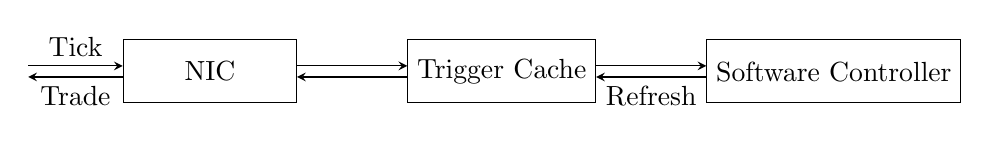
\begin{tikzpicture}[
    box/.style={
	draw,
	minimum width=2.2cm,
	minimum height=0.8cm
    },
    >=stealth
]
	\node[box] (nic) {NIC};
	\node[box, right=1.4cm of nic] (cache) {Trigger Cache};
	\node[box, right=1.4cm of cache] (controller) {Software Controller};

	% Tick / Trade
	\coordinate (tick) at ([xshift=-1.2cm,yshift=2pt]nic.west);
	\coordinate (trade) at ([xshift=-1.2cm,yshift=-2pt]nic.west);

	\draw[->] (tick) -- ([yshift=2pt]nic.west)
	    node[midway,above]{Tick};

	\draw[->] ([yshift=-2pt]nic.west) -- (trade)
	    node[midway,below]{Trade};

	% NIC <-> Trigger Cache
	\draw[->] ([yshift=2pt]nic.east) -- ([yshift=2pt]cache.west);
	\draw[->] ([yshift=-2pt]cache.west) -- ([yshift=-2pt]nic.east);

	% Trigger Cache <-> Software Controller
	\draw[->] ([yshift=2pt]cache.east) -- ([yshift=2pt]controller.west);
	\draw[->] ([yshift=-2pt]controller.west) -- ([yshift=-2pt]cache.east)
	    node[midway,below]{Refresh};
\end{tikzpicture}
\vspace{0.05cm}

An onboard \textbf{trigger cache} lets us store parameters to determine how to respond to market data.

Precomputing these before the latency-critical moment reduces hotpath latency.

However, because of the large volume of market data and limited space in the trigger cache, \textbf{tick-to-config} latency/throughput are still important considerations, especially considering `burstiness' of market data.

The cases when wire-to-wire matters most (low jitter) are often cases where marginal gains are going to be not that useful. On the other hand, large improvements can still have large impact if we begin to be consistently faster than some competitor.

\sectiondiagram{hardware}
\sectionquote{``All great events hang by a hair.'' Napoleon}
\section{Hardware Design}

\subsection{Field Programmable Gate Arrays}
Xilinx introduced the first FPGA in 1985. Xilinx was acquired by AMD in 2022.
\begin{center}
	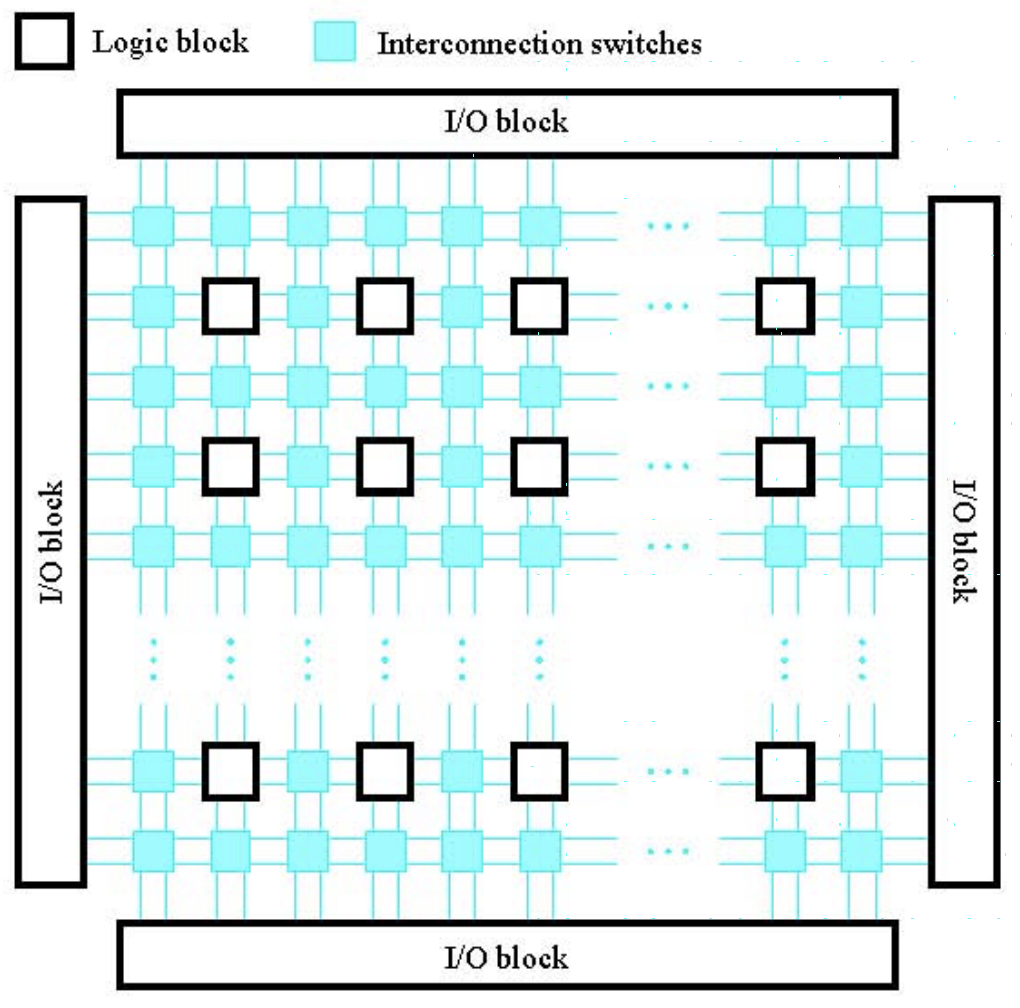
\includegraphics[scale=0.3]{assets/fpga.png}
\end{center}
While primarily useful onboard a NIC, FPGAs also have applications in other low-latency/high-throughput situations.

\subsection{Configurable Logic Blocks (CLBs)}
\begin{center}
	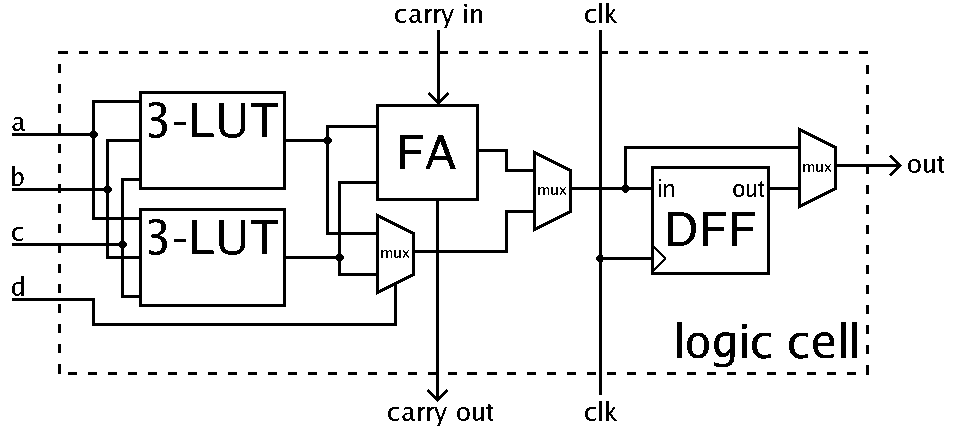
\includegraphics[scale=0.35]{assets/clb.png}
\end{center}

Different FPGAs will have different resources available in the CLB.

For instance, the \href{https://docs.amd.com/r/en-US/Alveo-X3522PV-Adaptable-Accelerator-Card-User-Guide-UG1607/}{AMD Alveo X3522 NIC} uses \href{https://docs.amd.com/r/en-US/ug574-ultrascale-clb/CLB-Resources}{UG574 UltraScale+ CLBs}.

\subsection{Synchronous Design}
Synchronous design involves updating \textbf{registers} according to \textbf{combinational functions} on each \textbf{clock edge}.

\newsavebox\lstA
\begin{lrbox}{\lstA}
\begin{lstlisting}[ basicstyle=\ttfamily\bfseries\scriptsize ]
module itch_volume #(
    parameter int NUM_STOCKS = 4
) (
    input logic clk, input logic valid,
    input logic [5:0] pos, input logic [7:0] data_byte,

    input logic [31:0] buy_threshold  [NUM_STOCKS],
    input logic [31:0] sell_threshold [NUM_STOCKS],

    output logic [31:0] buy_volume  [NUM_STOCKS],
    output logic [31:0] sell_volume [NUM_STOCKS],

    output logic buy_trigger,
    output logic sell_trigger,
    output logic [15:0] trigger_locate
);
\end{lstlisting}
\end{lrbox}
\href{https://edaplayground.com/x/9qhM}{\usebox{\lstA}}%Packet slicing, only read part of packet. Concept of a HDL

The length of each \textbf{clock cycle} must be chosen so that data has time to propagate to the destination register. %Reduce complexity of each step

\textbf{Clock domain crossings} must be separated by a specialised interface to avoid data corruption. %restricted by line bandwidth in some ways

\subsection{Parallelism}
A single clock cycle permits simultaneous dataflow through multiple CLBs at once.

Module latency will be equal to the number of clock cycles to produce an output, divided by the clock frequency.

One extreme example of parallelism afforded by special-purpose circuitry is a \href{https://docs.google.com/spreadsheets/d/1ndaz7_nyNNiciWW2bAGFsjldRJw72Wh_dNt0qzXUdKs/}{\textbf{systolic array}}.

%comment/diagram on DAGs and critical paths

\subsection{Memory}
A \textbf{D-Flip Flop} emits a binary signal when powered, equal to its data input on the most recent \textbf{clock edge}.
\begin{center}
	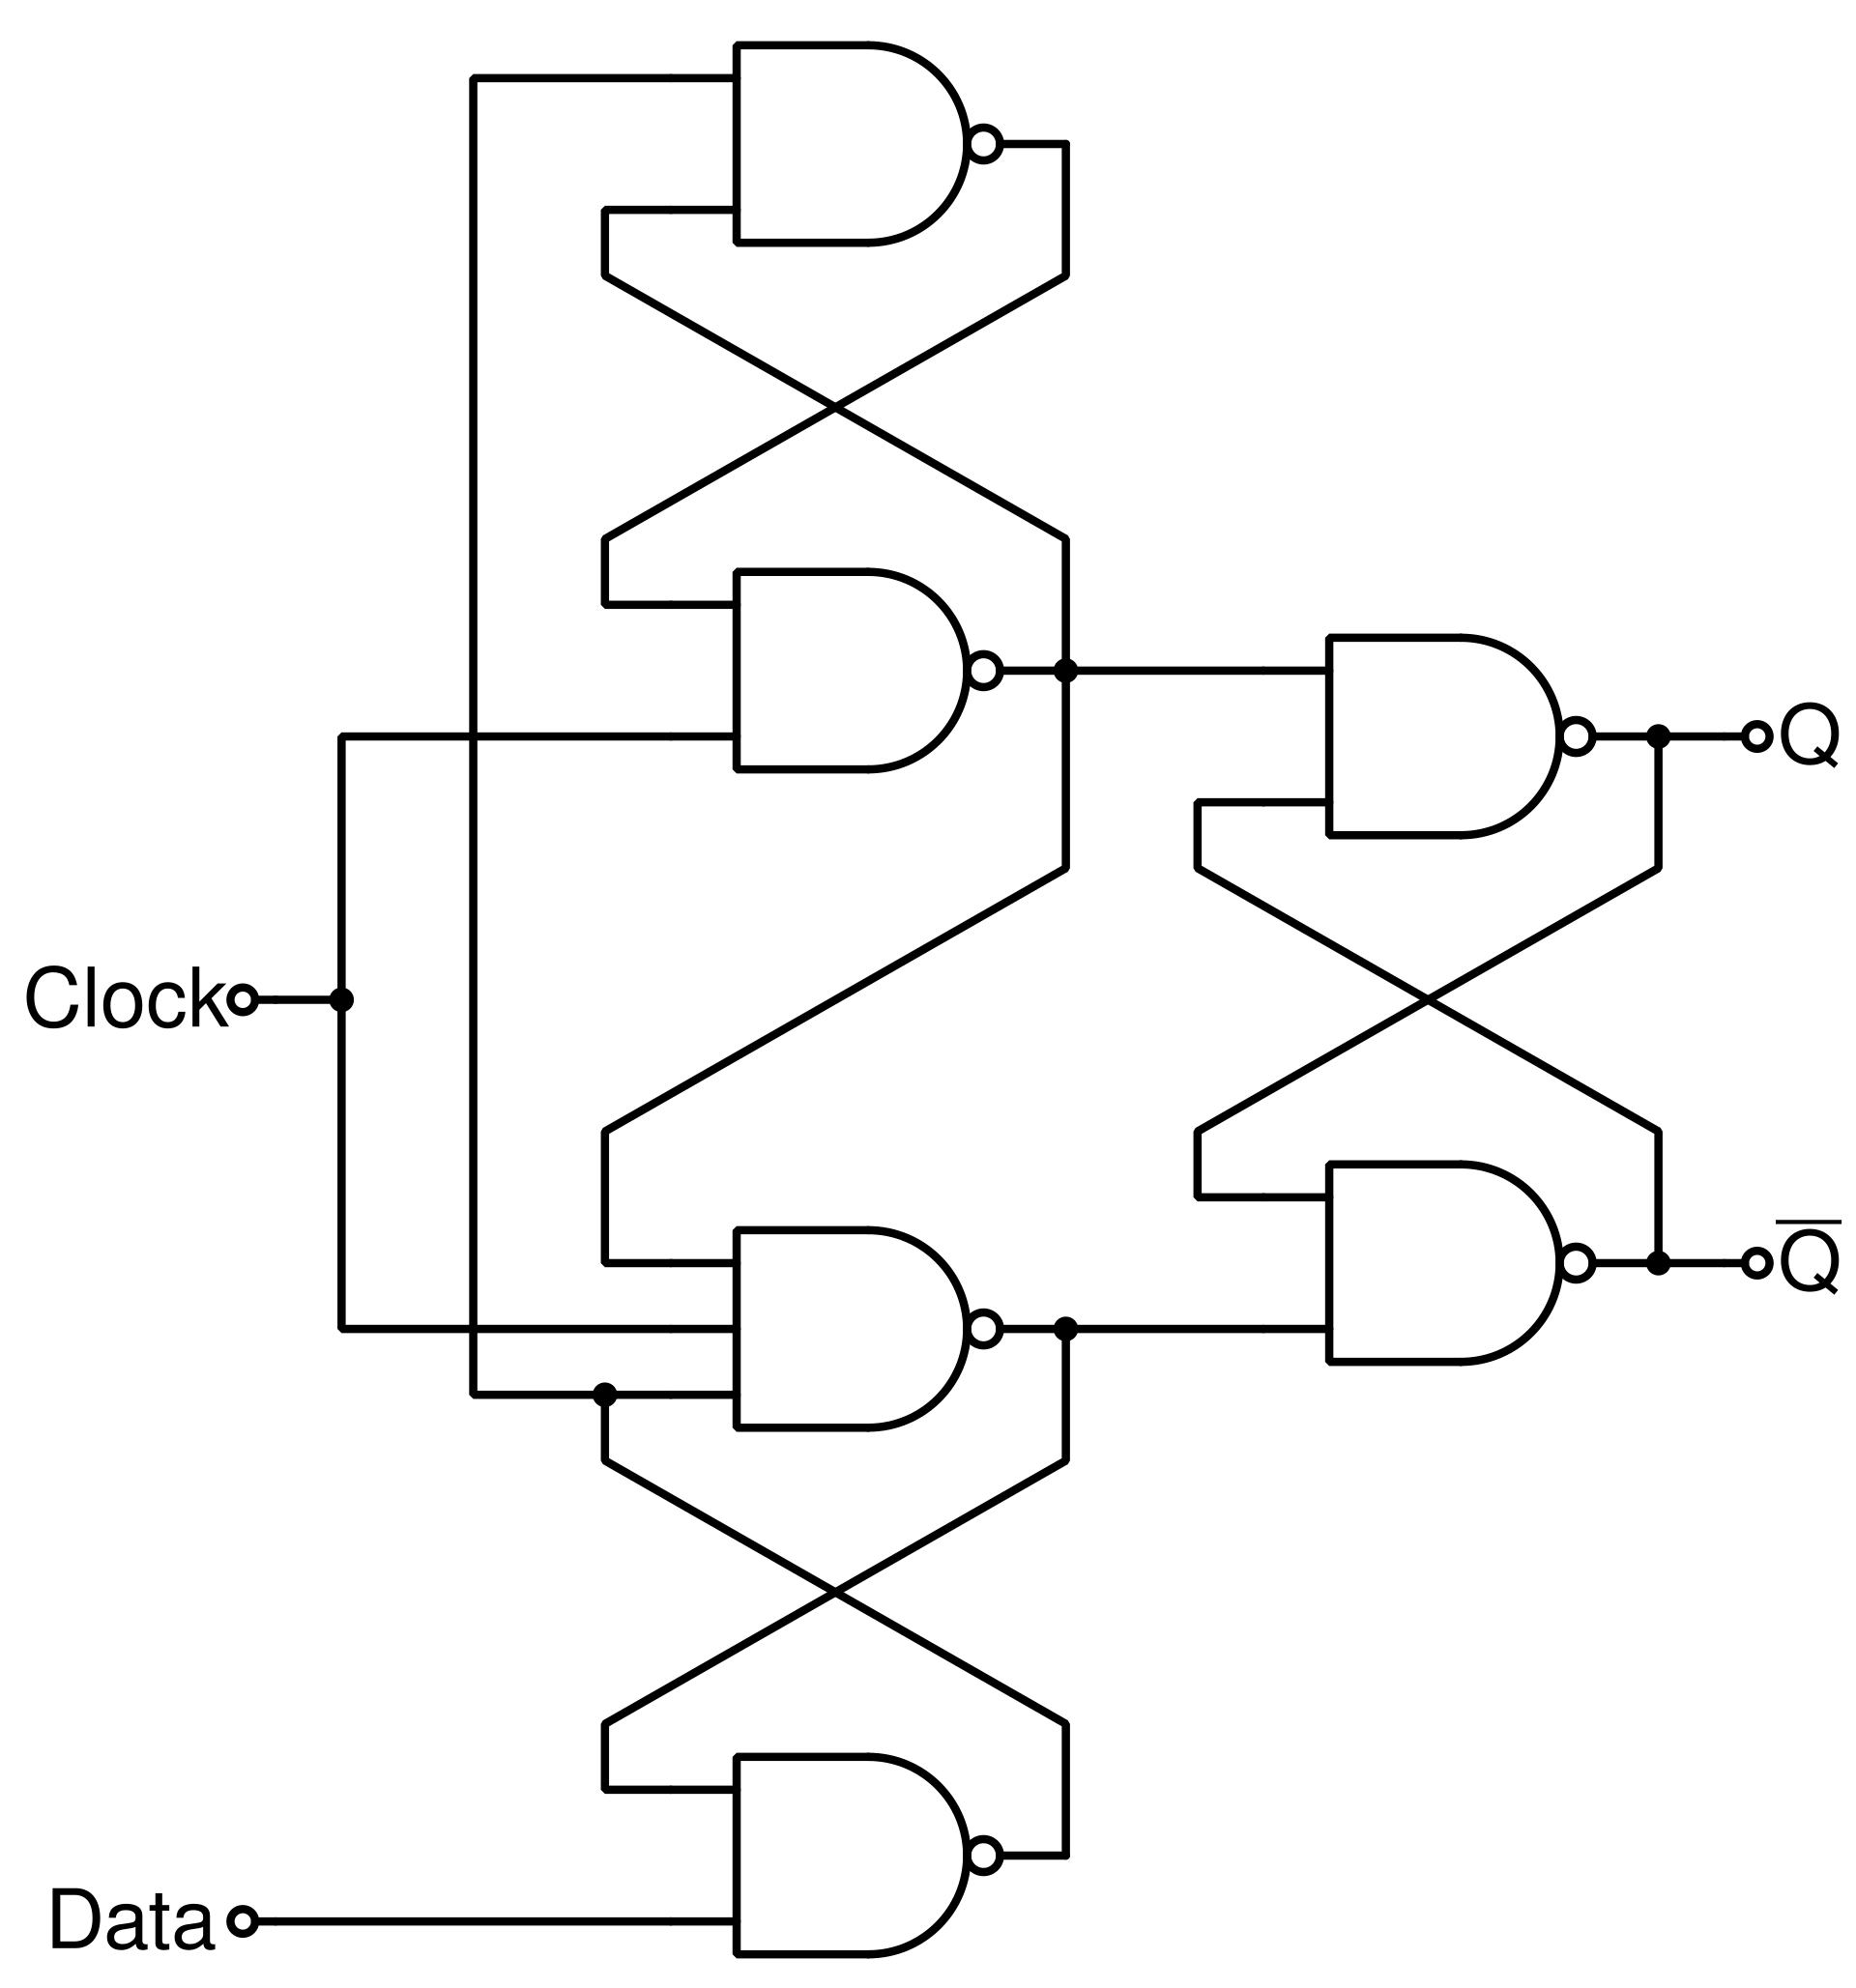
\includegraphics[scale=0.07]{assets/dflipflop.png}
\end{center}

\textbf{Block RAM} (B-RAM) is typically included in the FPGA fabric.

\begin{lstlisting}[ basicstyle=\ttfamily\bfseries\scriptsize ]
module ram #(parameter int ADDR_WIDTH = 16, parameter int DATA_WIDTH = 64) (
	input logic clk,
	input logic write,
	input logic [ADDR_WIDTH-1:0] address,
	input logic [DATA_WIDTH-1:0] data,
	output logic [DATA_WIDTH-1:0] read
);
\end{lstlisting} %might have multiple read/write ports

B-RAM is a kind of \textbf{Static Random Access Memory} (S-RAM). Dedicated RAM devices are typically cheaper, slower \textbf{Dynamic Random Access Memory} (D-RAM).

\begin{block}{RAM Timing}
	Some RAMs support \textbf{double data rate input/output} (DDIO), moving data at both positive and negative clock edges.

	Making a RAM block larger will generally necessitate slower timing. In theory, this is $O(\sqrt{N})$ for a 2-dimensional RAM layout.
\end{block}

\subsection{Synthesis}
Following design and verification, programming the board involves the following stages:
\begin{enumerate}
	\item Parsing of the \textbf{hardware description} (e.g. VHDL, Verilog, Clash, Hardcaml) into an abstract representation%minimal area is nice
	\item Identifying the dependency DAG of register values over time (\textbf{register-transfer level})
	\item Generating a \textbf{gate-level netlist}
	\item Translation into resources made available by the board, and optimising the placement of logic/routing for timing, power, etc. %also crosstalk
	\item Serialisation and `flashing' onto the board
\end{enumerate}
Optimisation generally makes use of some \textbf{cost model}. Depending on the software used, it may be non-deterministic.%intel quartus uses simulated annealing but vivado is in theory deterministic
%question. is it common to run out of resources

\subsection{High Level Synthesis (HLS)}
Sophisticated software also exists to translate \href{https://github.com/Xilinx/Vitis-HLS-Introductory-Examples/blob/master/Pipelining/Loops/pipelined_loop/loop_pipeline.cpp}{higher-level descriptions} (for instance, code written in a dialect of C) into RTL designs.

\subsection{Interconnects and PCIe (Peripheral Component Interconnect Express)}
\textbf{PCIe} is the standard way for specialised components (NIC, GPU, etc.) in a computer to communicate with the CPU.%also provides power

\begin{center}
	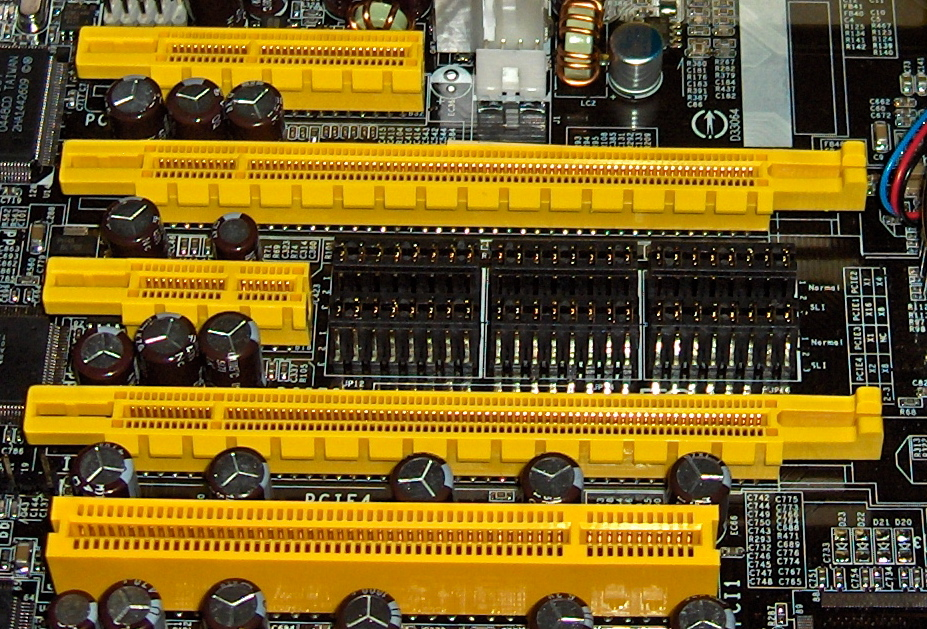
\includegraphics[scale=0.15]{assets/pcie.jpg}
\end{center}

OS/BIOS find components at startup and give them a \texttt{Bus:Device.Function} (BDF) address.

A clock signal is distributed from a central source for syncing.

Information is packetised, with packets carrying \href{https://docs.amd.com/r/en-US/pg194-axi-bridge-pcie-gen3/PCIe-Transaction-Type}{transactions}, which can be reads, writes, interrupts etc.

\sectiondiagram{software}
\sectionquote{``You don't need to be an engineer to be a racing driver, but you do need Mechanical Sympathy.'' Jackie Stewart}
\section{Software Design}
Hardware is expensive to buy, expensive to program, expensive to maintain. 

\subsection{Von Neumann Architecture}
\begin{block}{}
	``In analyzing the functioning of the contemplated device, certain classificatory distinctions suggest themselves immediately. \ldots

	\begin{itemize}
	\item A \textbf{central arithmetical part} of the device will probably have to exist, and this constitutes the first specific part \ldots

	\item Second: The logical control of the device, that is the proper sequencing of its operations can be most efficiently carried out by a \textbf{central control organ} \ldots

	\item Third: Any device which is to carry out long and complicated sequences of operations (specifically of calculations) must have a considerable \textbf{memory}.''
	\end{itemize}
	John Von Neumann, 1945
\end{block}

\subsection{CPUs}
Logically, a Central Processing Unit runs the following loop:
\begin{enumerate}
	\item \textbf{Fetch} the program instruction indicated by the \textbf{program counter}
	\item \textbf{Decode} the instruction into primitive operations %micro-operations
	\item \textbf{Execute} the instruction, which may involve:
	\begin{itemize}
		\item Computing some value
		\item Interacting with external \textbf{memory} (or cache)
		\item Altering the state of the CPU's \textbf{registers}
	\end{itemize}
\end{enumerate}

The \textbf{Instruction Set Architecture} (ISA) defines how \href{https://godbolt.org/z/e3q4rox9e}{\textbf{machine instructions}} are interpreted.

You can check what CPU you have with \texttt{lscpu}.

\subsubsection{Overclocking}
The Fetch-Decode-Execute loop requires some number of clock cycles for each instruction.

Naively, the amount of time a CPU takes to achieve a task will be the total number of clock cycles required times the clock period.

For maximum performance, CPUs can be \textbf{overclocked} relative to the speed they are designed for.

This generates heat in excess of what the CPU is designed to handle, so an appropriate \textbf{cooling system} is required.%not great if the rack is packed with stuff

It also increases the \textbf{power draw} of the system.

Clock frequency can be monitored using \texttt{turbostat}, e.g. \texttt{sudo turbostat -{}-quiet -{}-show Core,CPU,Busy\%,Bzy\_MHz,Avg\_MHz,IPC}.

OS-level control of clock frequency can be configured using \texttt{cpupower}.
%https://www.blackcoretech.com/

\subsubsection{Performance Optimisation}
\begin{itemize}
	\item Make sure to \textbf{do as little work as possible}
	\item Schedule tasks in a way that lets you \textbf{have many going at once}
	\item Arrange memory so you can get away with \textbf{communicating as little as possible}
	\item Use profiling tools to \textbf{constantly measure and compare}
\end{itemize}

\subsubsection{Microarchitecture}
\begin{center}
	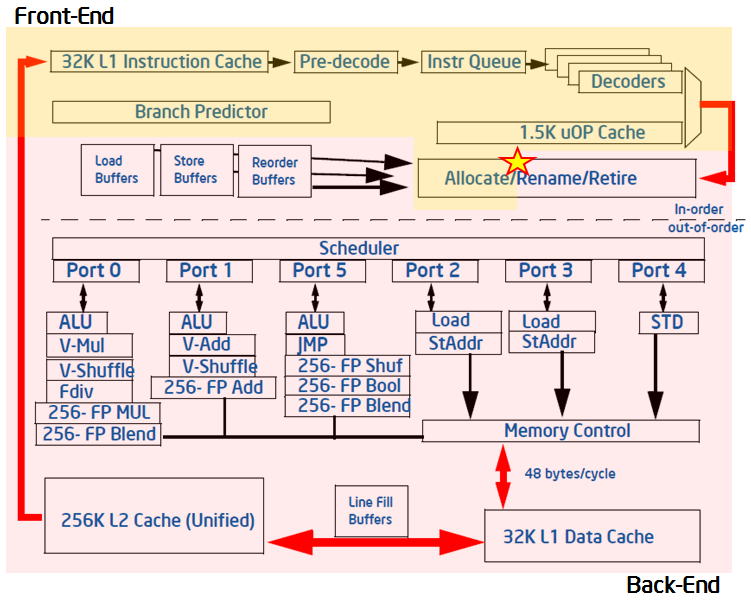
\includegraphics[scale=0.5]{assets/intel.png}
\end{center}
	
\subsubsection{Out-of-Order Execution}
\begin{block}{Parallelism}
	In practice, the Fetch-Decode-Execute loop is parallelised in modern CPUs.

	\begin{enumerate}
	\item \textbf{Issue} the instruction to a relevant \textbf{reservation station}
	\item Wait for the operands to be ready before \textbf{executing} the operation
	\item \textbf{Write} the result to the output register and \textbf{broadcast} to other reservation stations
	\end{enumerate}
\end{block}

Taking advantage of parallelism involves \textbf{dependency minimisation}. Modern compilers are quite good at this.

CPUs are not always transparent about their inner workings. Tools like \href{https://godbolt.org/z/8P6jKv81c}{\texttt{llvm-mca --timeline}} can give some very rough hints.

	%picture?
%https://en.wikipedia.org/wiki/Register_renaming#Out-of-order

	%https://www.jsulz.com/2020/02/19/everything-in-its-right-place-a-primer-on-hardware-support-for-high-performance-computer-architecture/
	%prf vs rat, renaming/virtual registers
	%memory order buffer / load-store queue

\subsection{x86}
An \textbf{Instruction Set Architecture} defines the available \textbf{machine instructions} and their behaviour.

The ISA also exposes a fixed set of \href{https://en.wikibooks.org/wiki/X86_Assembly/X86_Architecture}{\textbf{logical registers}}.

\begin{block}{x86}
	\begin{itemize}
	\item ISA developed by Intel in 1978, largely backwards-compatible
	\item Variable-length instructions%denser code packing
	\item Instructions often implemented using microoperations ($\mu$ops)
	\item Support for Single Instruction Multiple Data (SIMD)
	\end{itemize}
\end{block}

\subsection{Storing Local Variables}
\begin{block}{Register Spilling}
	Having many variables in scope can lead to \textbf{register pressure}

	To cope with this, variables may be \href{https://godbolt.org/z/6Mcdac7qY}{\textbf{spilled}} onto \textbf{stack memory}.
\end{block}

\subsubsection{Stack Memory}
A fixed amount of stack memory is allocated when the program starts.

The \textbf{stack pointer} (\texttt{rsp} on x86) represents the region of data used in a function scope.

x86 supports \texttt{push} and \texttt{pop} operations.

At the start of a function call:
\begin{itemize}
\item Registers that will be used are pushed to stack
\item Register \texttt{rsp} is decremented by the space required for storing local variables
\end{itemize}

Moving \texttt{rsp} outside the allocated range of stack memory represents a \href{https://godbolt.org/z/85TTjWKq7}{\textbf{stack overflow}}.

\begin{center}
	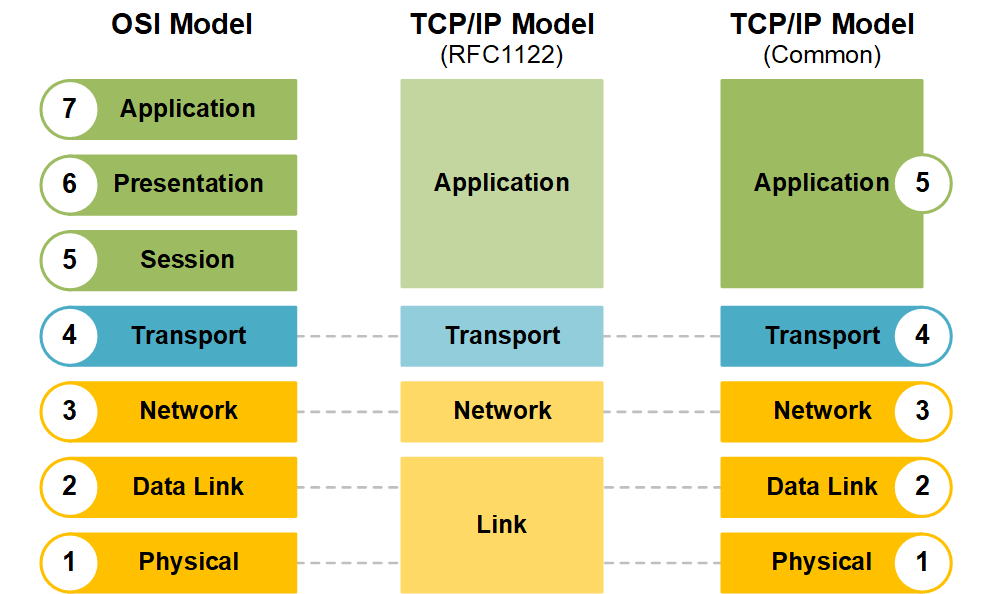
\includegraphics[scale=0.2]{assets/stack.png}
\end{center}

\subsubsection{Heap Memory}
Sometimes the amount of memory we need is only known at runtime.

We can request \textbf{virtual memory} from the OS using syscalls like \texttt{brk} and \texttt{mmap}.

Since syscalls are expensive, we can use a software-level allocator like \texttt{malloc} that fetches a large amount of memory in advance.

Allocation is still expensive and should be avoided in the hotpath.

\textbf{Heap fragmentation} and \textbf{pressure} can slow down allocation even further.

Mapping of pointers to physical memory addresses relies on the \textbf{translation lookaside buffer}.

\subsection{Caching}
Register access is much faster than RAM access.

\textbf{Caches} provide intermediate \textbf{access speeds} and \textbf{memory capacity} by \textbf{cache lines}.

Caches use \href{https://uops.info/cache.html}{\textbf{eviction rules}} (e.g. Least Recently Used) to determine which data to keep in memory. %makes sense for stack

Caches are organised \textbf{hierarchically}: L1, L2, L3 (+ RAM, swap space).

\textbf{Cache misses} are more expensive.

Cache details are shown by \texttt{lscpu}.

\subsubsection{Cache Misses}
Here's the distribution we get if we measure how long it takes to access a random pointer:
\begin{center}
	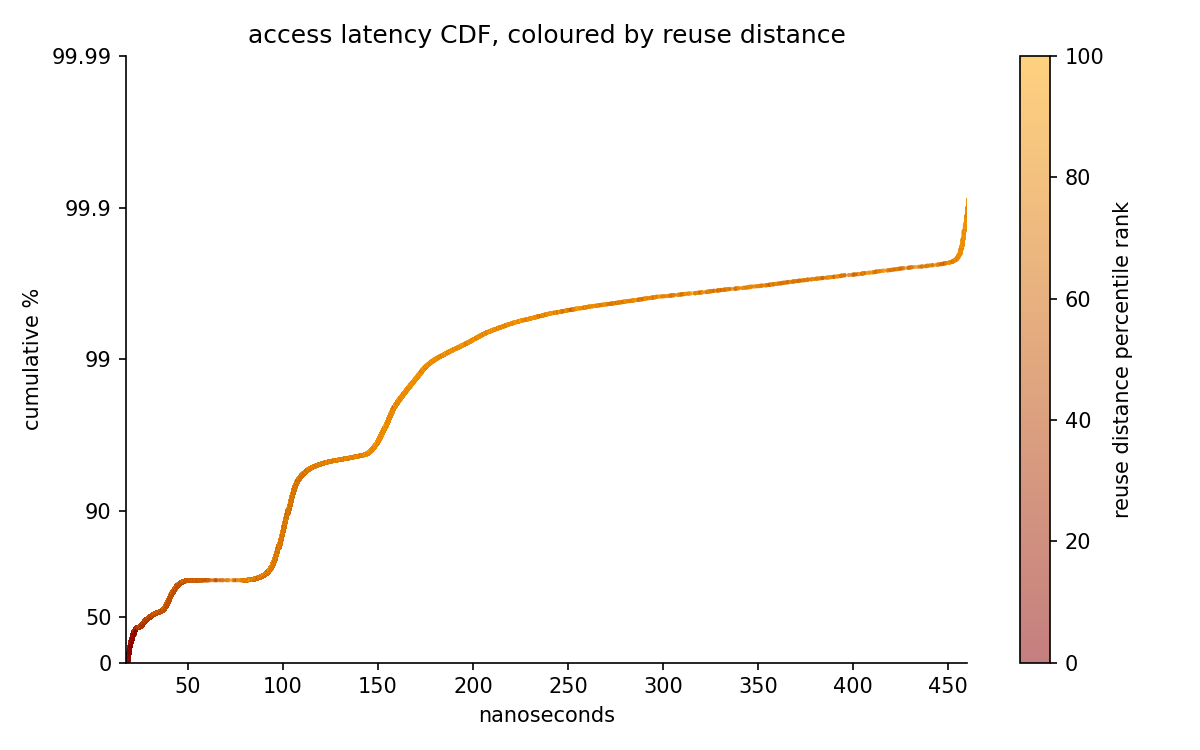
\includegraphics[scale=0.45]{code/cache/cdf.png}
\end{center}
This looks like a mixture distribution, and in principle the components represent different cache levels with different access latency distributions.

Cache misses can be avoided by controlling:
\begin{itemize}
	\item data size
	\item data layout
	\item access patterns
\end{itemize}

Instruction cache misses can also be reduced by avoiding jumps, e.g. through function inlining.

%alignment. how to ensure
%prefetching, prefetch-friendly programming

\subsubsection{Cache-Friendly Design}
We can run some experiments here. Suppose we want to look up whether an item appears in a container. The time this takes might depend on how big the container is.
\begin{center}
	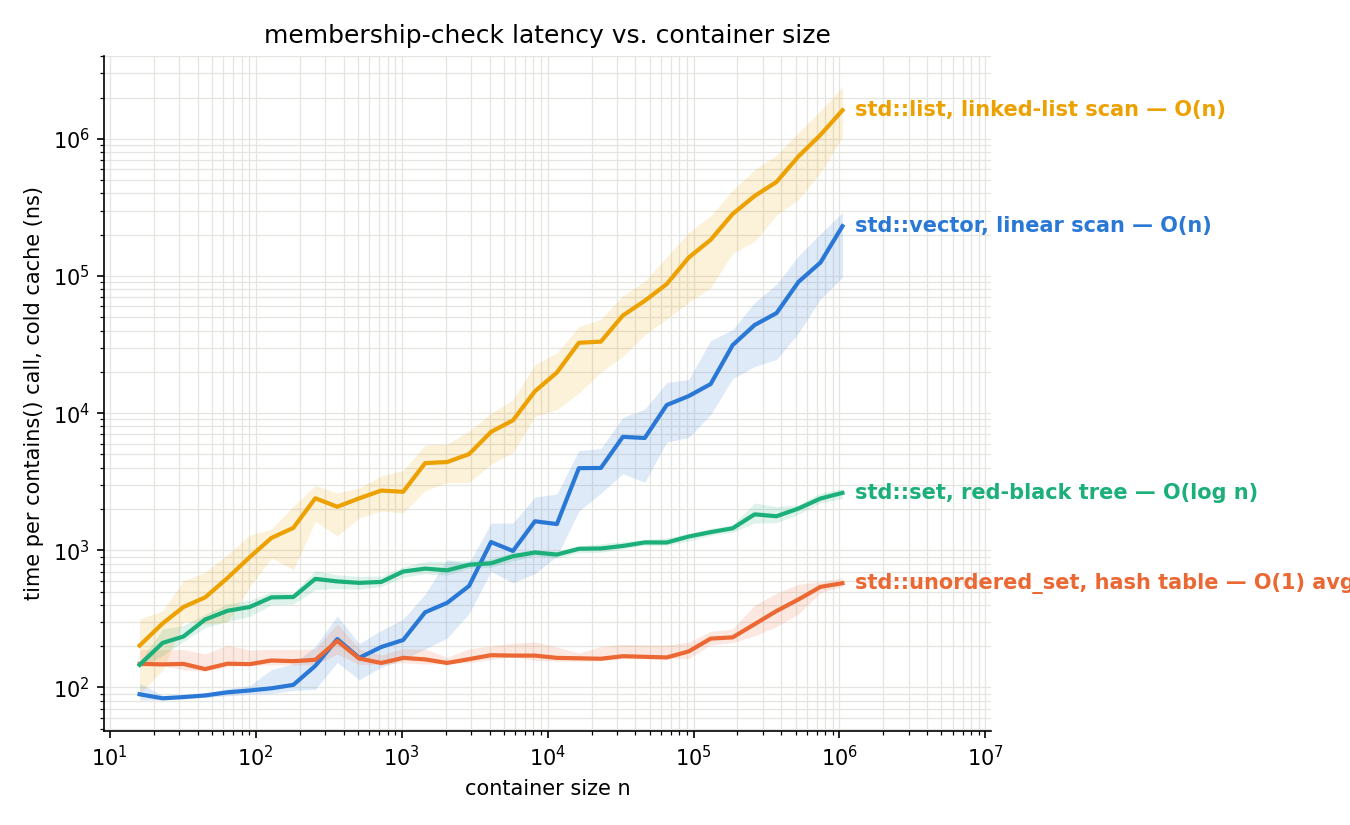
\includegraphics[scale=0.5]{code/container/container_latency.png}
\end{center}
We can see that even for hundreds of elements, the vector implementation outperforms, despite having worse time complexity. Linked list is the worst, since we have no guarantee of a contiguous memory layout.

\subsection{Branch Prediction}
Often the program counter needs to \textbf{jump} depending on some condition.

In order to allow pipelining before this condition is resolved, CPUs use \textbf{speculative execution} based on a \textbf{branch predictor}.

\begin{block}{Branch Prediction Rules}
	\begin{itemize}
	\item Static: always jump, jump if backwards
	\item Local history: last outcome, saturating counter
	\item Global history
	\item Random
	\item Learned: perceptron, hash buckets, etc.
	\end{itemize}
\end{block}

We can run some experiments here. Suppose we process random data that is uniformly distributed between 0 and 1. We branch according to whether this data exceeds $x$. Branch predictability, and therefore latency, will be a function of $x$.
\begin{center}
	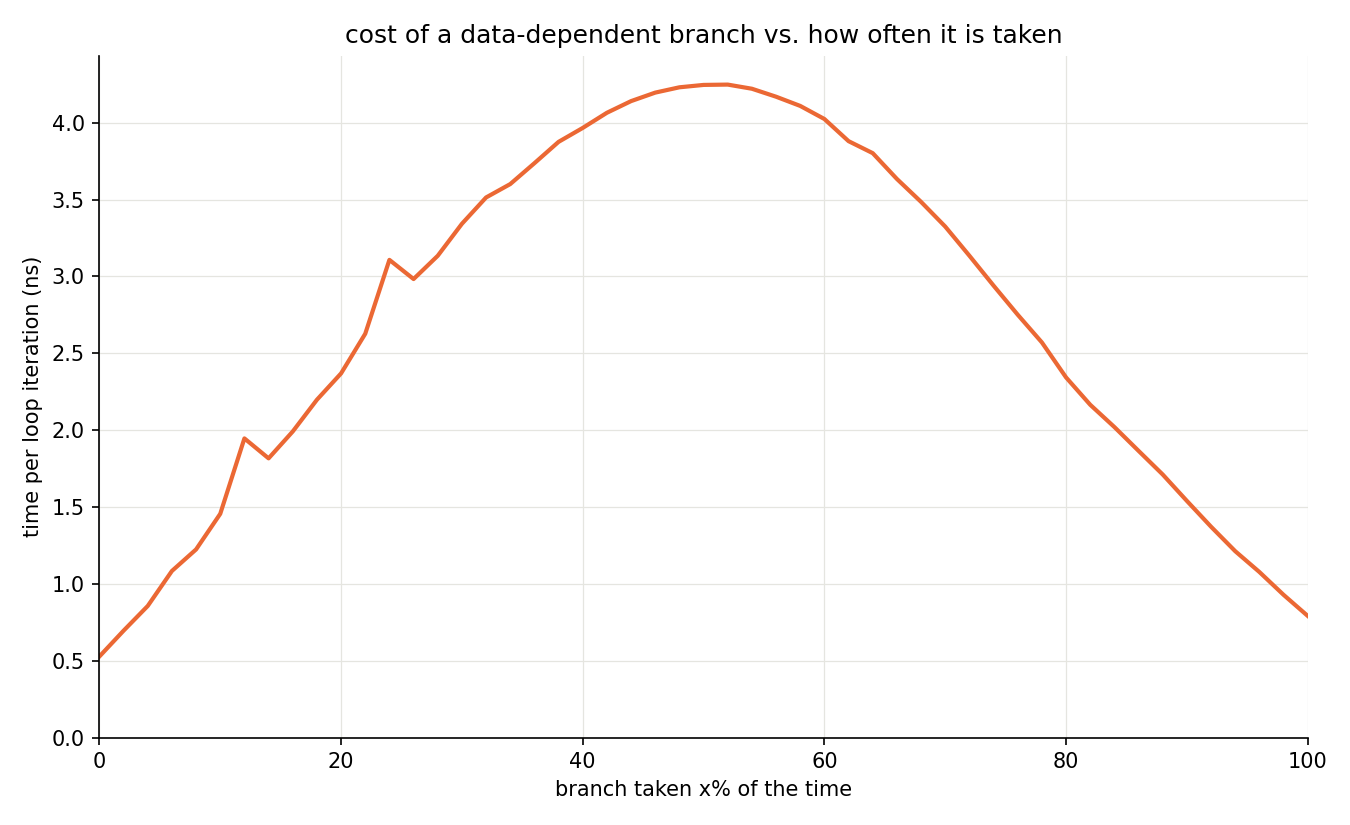
\includegraphics[scale=0.4]{code/branch/branch_latency.png}
\end{center}

\subsubsection{Branch Misses}
We can count branch misses with \texttt{perf stat -e branches,branch-misses}. This relies on the CPU's Performance Monitoring Unit (PMU) counters.

Figuring out which branches were mispredicted can be nontrivial and quite CPU-specific.

Sometimes it is cheaper to compute both branches and use \texttt{cmov}.

We can hint to the compiler with keywords like \texttt{[[likely]]}/\texttt{[[unlikely]]}. Instruction-level branch hints are not normally supported.
%"Time forks perpetually toward innumerable futures." Borges

\subsection{Profiling Tools}
\begin{itemize}
	\item \texttt{time} / \href{https://github.com/sharkdp/hyperfine}{\texttt{hyperfine}}
	\item \texttt{perf}
	\item \texttt{ftrace}
	\item \href{https://www.brendangregg.com/FlameGraphs/cpu-bash-flamegraph.svg}{\texttt{flamegraphs}}
	\item \href{https://github.com/janestreet/magic-trace}{\texttt{magic-trace}}
	\item \texttt{valgrind --tool=cachegrind}, \href{https://github.com/david-grs/papipp}{\texttt{libpapi}}
	\item \texttt{hwlatdetect}
	\item \texttt{rteval}, \texttt{osnoise}
	\item \texttt{\_\_rdtsc()} + \texttt{\_mm\_lfence()}
\end{itemize}

\subsection{Multi-Core Processing}
Modern processors come equipped with multiple \textbf{cores}.

Each core may have multiple CPUs, visible with \texttt{lscpu -e=CPU,CORE}.

Each CPU can execute instructions independently, e.g. for multithreaded code.

Threads may be \textbf{pinned} to a core, or have an \textbf{affinity bitmask} (\texttt{taskset}, \texttt{cpuset}, \texttt{tuna}).

\textbf{Interrupt Request} (IRQ) affinity (particularly NIC IRQs) and steering may assist performance.

Configuration parameters like \texttt{isolcpus} and \texttt{nohz\_full} allow a core to avoid running certain tasks.

\subsection{Interprocess Communication (IPC)}
Different processes often need to communicate information to one another.

Libraries like \texttt{boost::interprocess} rely on the \texttt{mmap} syscall to allocate \textbf{shared memory}.

\subsubsection{Cache Coherence}
Each \textbf{cache line} is \textbf{single-writer} to ensure \textbf{coherence}. Transferring ownership is costly.

Threads modifying data in the same cache line causes ownership to `bounce' between cores. This is sometimes known as \textbf{false sharing}, particularly when the data is only coincidentally on the same cache line.

Cache writes trigger \textbf{cache invalidation} for other cores reading the cache line.

It may be possible to configure the NIC to share a cache with the processors.

\begin{block}{}
	``There are 2 hard problems in computer science: cache invalidation, naming things, and off-by-1 errors.'' Leon Bambrick
\end{block}

\subsubsection{Race Conditions}
Even with single-writer, \textbf{data races} are still possible if operations are \textbf{non-atomic}. Using a \textbf{mutex} also prevents this.

\begin{lstlisting}[ basicstyle=\ttfamily\bfseries\scriptsize ]
mov    eax, DWORD PTR [x]    ; load x
add    eax, 1                ; x + 1
mov    DWORD PTR [x], eax    ; store x
\end{lstlisting}

The atomic version would be:
\begin{lstlisting}[ basicstyle=\ttfamily\bfseries\scriptsize ]
lock add DWORD PTR [x], 1
\end{lstlisting}

A \textbf{producer-consumer} queue can help prevent data races and balance load across threads.

\subsection{Multitasking}
OS multitasking is achieved using:
\begin{itemize}
	\item A \textbf{priority mechanism}, set using \texttt{chrt}\footnote{e.g. \texttt{sched\_other}/\texttt{sched\_normal}, \texttt{sched\_batch}, \texttt{sched\_fifo}, \texttt{sched\_rr}, \texttt{sched\_deadline}}
	\item A \textbf{task-switching mechanism}, e.g. time slicing, blocks/yields, interrupts
\end{itemize}

\begin{block}{Types of Multitasking}
	Multitasking governs both \textbf{multiprocessing} or \textbf{multithreading} (e.g. \texttt{std::thread}).

	Alternatively, userspace multitasking can be achieved using \textbf{coroutines} or similar constructs (e.g. \texttt{boost::fibers::fiber}).
\end{block}

Task switching is relatively expensive.

Interrupt-based communication should generally be avoided, e.g. with \texttt{IRQBALANCE\_BANNED\_CPUS}.%interrupt storms

\subsection{Kernel Networking}
\begin{center}
	\href{https://godbolt.org/z/6ejP5K4o8}{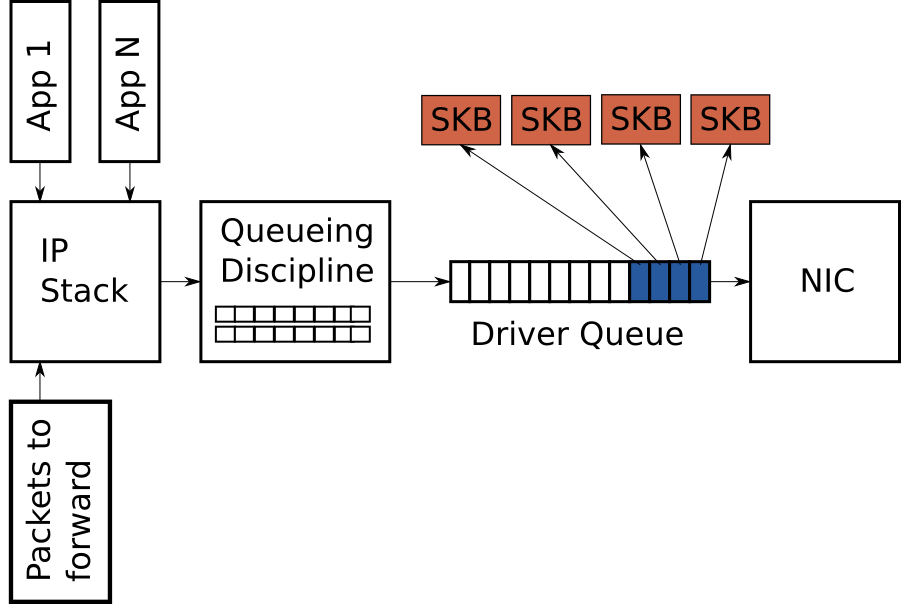
\includegraphics[scale=0.4]{assets/kernel_tx.png}}
\end{center}

This can be profiled at a high level with tools like \texttt{sockperf}.

\subsection{Userspace Networking}
Interrupt-based networking introduces \textbf{task-switching overhead}.

A standard NIC setup will \textbf{not interrupt immediately} upon receipt of a message.

We can \texttt{mmap} the NIC's DMA segment to use \textbf{shared memory} instead.

\textbf{Continuous polling} of the RX queue allows for rapid response. We can also do this with any other data we might need at processing time to `warm' the relevant cache line.

\begin{block}{Kernel Bypass Frameworks}
	We need to know the layout of DMA to communicate with the NIC.

	TCPDirect, DPDK (+F-Stack/mTCP) provide specialised APIs for this.

	OpenOnload and Nvidia Messaging Accelerator make use of \texttt{LD\_PRELOAD} to monkeypatch\footnote{Specifically, changing the dynamic linking} \texttt{libc}'s socket calls.
\end{block}

\sectiondiagram{program}
\sectionquote{``There is no science apart from the general. \\ It may even be said that the very object of the exact sciences is to spare us these direct verifications.'' Henri Poincaré}
\section{Programming}

\subsection{High-Level Languages}
C, C++, Rust, OCaml, Go, Python, etc.
\begin{itemize}
	\item Safety, e.g. types %Knight capital group
	\item Brevity, e.g. \texttt{a+b+c+d}
	\item Automation, e.g. \texttt{f()}
	\item Portability\footnote{Exceptions: compiler pragmas, inline assembly, OS-specific libraries, undefined behaviour, etc.}
	\item Metaprogramming, e.g. \texttt{template}
	\item \textbf{Speed of iteration}
\end{itemize}

Code performance and code quality are often in tension.

\subsection{Abstraction}
\begin{block}{}
	``C++ leads to really really bad design choices. You invariably start using the "nice" library features of the language like STL and Boost and other total and utter crap, that may "help" you program, but causes:
	\begin{itemize}
	\item infinite amounts of pain when they don't work (and anybody who tells me that STL and especially Boost are stable and portable is just so full of BS that it's not even funny)
	\item inefficient abstracted programming models where two years down the road you notice that some abstraction wasn't very efficient, but now all your code depends on all the nice object models around it, and you cannot fix it without rewriting your app.
	\end{itemize}
	In other words, \textbf{the only way to do good, efficient, and system-level and portable C++ ends up to limit yourself to all the things that are basically available in C}.'' Linus Torvalds
\end{block}

C++ is nice in the sense that you can basically just write C if you want to.

%correctness, testing and debugging

\subsection{Compilation}
\begin{block}{Development}
	Since compilation does work for us, it can take time on big projects. If we're only checking correctness, we can get away with less optimised machine code.

	\begin{itemize}
	\item Optimisation levels, \texttt{-O0} (default) to \texttt{-O3}, \texttt{-Os}, \texttt{-Oz}, \texttt{-Og}, \texttt{-Ofast}
	\item Dynamic linking and \texttt{Makefile}s (vs. \href{https://llvm.org/docs/LinkTimeOptimization.html}{link time optimisation})
	\end{itemize}

	Compilers can interfere with profiling by eliminating unused components.
\end{block}

\begin{block}{Production}
	Compilation frontloads a lot of computation and validation. It can find optimisations or errors that are not obvious.

	Appropriate compiler hints can help improve performance when the compiler is not so smart. Compilers might use a cost model we are not interested in or heuristics that are not suited to the problem at hand.
	%AST, compiler IR

	Some very smart compilers can do \textbf{profile-guided optimisation}.
\end{block}

\subsection{Time-to-Market}
Everything rots:
\begin{itemize}
	\item Alphas decay
	\item Competitors get faster
	\item Market structure changes
	\item Flow changes
\end{itemize}

What works now may not work tomorrow.

\begin{align*}
	\text{Team profitability} &= \text{Rate of Discovery} \times \text{Strategy Profitability} \\
	&\times (\text{Lifespan of Strategy} - \text{Time to Market})
\end{align*}

\subsection{Speed is Not Everything}
Speed is the one thing everyone wants.

Exorbitant investment in ultra-low-latency systems can quickly stop being useful if someone else becomes much faster.

Focusing on other aspects of the strategy can matter more:
\begin{itemize}
	\item Order management
	\item Predictive power
	\item Market impact
	\item Risk management and controls
	\item Human oversight
	\item Financing
\end{itemize}

\begin{block}{}
	``A strange game.

	The only winning move is not to play.'' WOPR
\end{block}

\part{Bibliography}
\section{Useful}
\begin{itemize}
	\item Databento. ``An introduction to matching engines.'' \textit{Databento Blog}, 26 August 2024. \url{https://databento.com/blog/introduction-matching-engines}
	\item Databento. ``Analyzing private fills and canary orders with Databento high-precision market data timestamps.'' \textit{Medium}, June 2024. \url{https://medium.databento.com/analyzing-private-fills-and-canary-orders-with-databentos-high-precision-market-data-timestamps-8cb12f82a1a3}
	\item Databento. ``How we serve real-time tick data of the entire US options market over the internet---on a single server.'' \textit{Databento Blog}, 25 March 2024. \url{https://medium.databento.com/how-we-serve-real-time-tick-data-of-the-entire-us-options-market-over-the-internet-on-a-single-db05f9198378}
	\item Ulrich Drepper. \textit{What Every Programmer Should Know About Memory}. Red Hat, 2007. \url{https://www.akkadia.org/drepper/cpumemory.pdf}
	\item Matt Godbolt. ``Advanced Skylake Deep Dive.'' Jane Street, YouTube, 23 December 2025. \url{https://www.youtube.com/watch?v=BVVNtG5dgks}
	\item Matt Godbolt. ``Benchmarking -- It's About Time.'' Keynote, C++Now 2026, YouTube, 14 July 2026. \url{https://www.youtube.com/watch?v=EU_nQh8wg5A}
	\item Iwona Kotlarska. ``Optimising Compiler Performance: A Case For Devirtualisation.'' \textit{HRTbeat}, Hudson River Trading, 21 May 2024. \url{https://www.hudsonrivertrading.com/hrtbeat/optimising-compiler-performance-a-case-for-devirtualisation/}
	\item The Linux Kernel Documentation. ``Reducing OS jitter due to per-cpu kthreads.'' \url{https://docs.kernel.org/admin-guide/kernel-per-CPU-kthreads.html}
	\item Luke Maurer. ``Finding memory leaks with Memtrace.'' \textit{Jane Street Tech Blog}, 6 October 2020. \url{https://blog.janestreet.com/finding-memory-leaks-with-memtrace/}
	\item Jonathan M\"uller. ``Cache-Friendly C++.'' CppCon 2025, YouTube, 29 December 2025. \url{https://www.youtube.com/watch?v=g_X5g3xw43Q}
	\item Nasdaq. \textit{Genium INET OMnet Message Reference for SGX}. Software version 5.0.50.x, document version SKROM\_a42, 29 January 2026. \url{https://api2.sgx.com/sites/default/files/2026-06/OMnet_MessRef_SGX_va42.pdf}
	\item Nasdaq. ``Options Order Feed.'' \url{https://www.nasdaq.com/Options_Order_Feed}
	\item Red Hat. ``Networking.'' In \textit{Red Hat Enterprise Linux 6 Performance Tuning Guide}, chapter 8. \url{https://docs.redhat.com/en/documentation/red_hat_enterprise_linux/6/html/performance_tuning_guide/main-network#s-network-future}
	\item Red Hat. ``Reducing CPU performance spikes.'' In \textit{Optimizing RHEL 8 for Real Time for Low Latency Operation}. \url{https://access.redhat.com/documentation/en-us/red_hat_enterprise_linux_for_real_time/8/html-single/optimizing_rhel_8_for_real_time_for_low_latency_operation/index#proc_reducing-cpu-performance-spikes_optimizing-RHEL8-for-real-time-for-low-latency-operation}
	\item Alexander Stephan and Lars W\"ustrich. ``The Path of a Packet Through the Linux Kernel.'' In \textit{Seminar Innovative Internet Technologies and Mobile Communications (IITM), WS 23}. Technical University of Munich, 2024. doi:10.2313/NET-2024-04-1\_16. \url{https://www.net.in.tum.de/fileadmin/TUM/NET/NET-2024-04-1/NET-2024-04-1_16.pdf}
	\item Synopsys. ``What is Synthesis?'' \textit{Synopsys Glossary}. \url{https://www.synopsys.com/glossary/what-is-synthesis.html}
\end{itemize}

\section{Interesting}
\begin{itemize}
	\item Marc Brooker. ``It's always \texttt{TCP\_NODELAY}. Every damn time.'' 9 May 2024. \url{https://brooker.co.za/blog/2024/05/09/nagle.html}
	\item Kevin Carpenter. ``Back to Basics: Custom Allocators Explained -- From Basics to Advanced.'' CppCon, YouTube, 12 February 2026. \url{https://www.youtube.com/watch?v=RpD-0oqGEzE}
	\item cocomelonc. ``Linux hacking part 4: Measuring cache hit and cache miss times in linux.'' 1 February 2025. \url{https://cocomelonc.github.io/linux/2025/02/01/linux-hacking-4.html}
	\item Stewart Denholm, Hiroaki Inoue, Takashi Takenaka, and Wayne Luk. ``Application-specific customisation of market data feed arbitration.'' In \textit{2013 International Conference on Field-Programmable Technology (FPT)}. IEEE, 2013. \url{https://ieeexplore.ieee.org/document/6718377}
	\item Emil Ernerfeldt. ``The Myth of RAM, part I.'' 21 April 2014. \url{https://www.ilikebigbits.com/2014_04_21_myth_of_ram_1.html}
	\item Tom Herbert. ``Hardware FIFOs --- Device queues edition.'' \textit{Medium}, December 2024. \url{https://tomaherbert.com/hardware-fifos-device-queues-edition-b7b4ec16b0a9}
	\item Tom Herbert. ``The alphabet soup of receive packet steering: RSS, RPS, RFS, and aRFS.'' \textit{Medium}, February 2025. \url{https://tomaherbert.com/the-alphabet-soup-of-receive-packet-steering-rss-rps-rfs-and-arfs-c84347156d68}
	\item Matt Hurd. ``The accidental HFT firm.'' \textit{Meanderful}, 24 January 2018. \url{https://meanderful.blogspot.com/2018/01/the-accidental-hft-firm.html}
	\item John Michael Huth. ``A Clear Market Fairness Issue Requires a Clear, Collective Response.'' \textit{RealClearMarkets}, 14 February 2018. \url{https://www.realclearmarkets.com/articles/2018/02/14/a_clear_market_fairness_issue_requires_a_clear_collective_response_103150.html}
	\item Intel. ``Top-down Microarchitecture Analysis Method.'' In \textit{Intel VTune Profiler Cookbook}, version 2024.1. \url{https://www.intel.com/content/www/us/en/docs/vtune-profiler/cookbook/2024-1/top-down-microarchitecture-analysis-method.html}
	\item Jane Street. ``System Jitter and Where to Find It: A Whack-a-Mole Experience.'' YouTube, 15 November 2024. \url{https://www.youtube.com/watch?v=I_TtMk5z0O0}
	\item David L. Mills. ``A Brief History of NTP Time: Memoirs of an Internet Timekeeper.'' \textit{ACM SIGCOMM Computer Communication Review} 33(2), 2003. \url{https://www.eecis.udel.edu/~mills/database/papers/history.pdf}
	\item John von Neumann. \textit{First Draft of a Report on the EDVAC}. Moore School of Electrical Engineering, University of Pennsylvania, 1945. \url{https://web.archive.org/web/20070623082626/http://qss.stanford.edu/%7Egodfrey/vonNeumann/vnedvac.pdf}
	\item Reuters. ``China curbs `flash boys' access to exchange data, sources say.'' 19 January 2026. \url{https://www.reuters.com/world/china/china-curbs-flash-boys-access-exchange-data-sources-say-2026-01-19/}
	\item David Schneider. ``Wall Street Tries Shortwave Radio to Make High-Frequency Trades Across the Atlantic.'' \textit{IEEE Spectrum}, 1 June 2018. \url{https://spectrum.ieee.org/wall-street-tries-shortwave-radio-to-make-highfrequency-trades-across-the-atlantic}
	\item Dan Siemon. ``Queueing in the Linux Network Stack.'' \textit{Linux Journal}, 2013. \url{https://www.coverfire.com/articles/queueing-in-the-linux-network-stack/}
	\item Sergey Slotin. ``Machine Code Analyzers.'' In \textit{Algorithms for Modern Hardware}. Algorithmica, 2022. \url{https://en.algorithmica.org/hpc/profiling/mca/}
	\item Jake Yoon. ``The World's Fastest Matching Engine Algorithm.'' arXiv:2606.01183, 2026. \url{https://arxiv.org/abs/2606.01183}
\end{itemize}
\end{document}

